\documentclass[12pt]{article}


\usepackage[margin=1.1in,footskip=.25in]{geometry}

\usepackage{tabularx}
\usepackage[table]{xcolor}
\usepackage{multirow}

\usepackage{listings}
\usepackage{xcolor}
\usepackage{color}

\usepackage{verbatim}

\definecolor{dkgreen}{rgb}{0,0.6,0}
\definecolor{gray}{rgb}{0.5,0.5,0.5}
\definecolor{mauve}{rgb}{0.58,0,0.82}
 
\definecolor{codegreen}{rgb}{0,0.6,0}
\definecolor{codegray}{rgb}{0.5,0.5,0.5}
\definecolor{codepurple}{rgb}{0.58,0,0.82}
\definecolor{backcolour}{rgb}{0.95,0.95,0.92}



\lstdefinestyle{mystyle}{
    commentstyle=\color{codegreen},
    keywordstyle=\color{magenta},
    numberstyle=\tiny\color{codegray},
    stringstyle=\color{codepurple},
    basicstyle=\ttfamily\normalsize,
    breakatwhitespace=false,         
    breaklines=true,                 
    captionpos=b,                    
    keepspaces=true,                              
    showspaces=false,                
    showstringspaces=false,
    showtabs=false,                  
    tabsize=3
}

\lstset{style=mystyle}

\newcolumntype{C}{ >{\centering\arraybackslash} m{5cm} }
\newcolumntype{E}{ >{\centering\arraybackslash} m{7cm} }
\newcolumntype{D}{ >{\centering\arraybackslash} m{3cm} }
\newcolumntype{F}{ >{\centering\arraybackslash} m{1cm} }

\usepackage{array}

\usepackage{tikz} 
\usetikzlibrary{graphs,quotes,arrows.meta}
\usetikzlibrary{automata}
\usetikzlibrary{positioning}
\usetikzlibrary{patterns}
\usetikzlibrary{matrix,backgrounds}
\usetikzlibrary{arrows,shapes,trees}
\usetikzlibrary{chains}
\usetikzlibrary{calc}


\tikzstyle{vertex}=[draw,fill=black!5,circle,minimum size=20pt,inner sep=1pt]
\tikzstyle{error}=[fill=red!60]

\tikzset{
  treenode/.style = {align=center, inner sep=0pt, text centered,
    font=\sffamily},
  arn_n/.style = {treenode, circle, white, font=\sffamily\bfseries, draw=black,
    fill=black, text width=1.5em},% arbre rouge noir, noeud noir
  arn_r/.style = {treenode, circle, red, draw=red,
    text width=1.5em, very thick},% arbre rouge noir, noeud rouge
  arn_x/.style = {treenode, rectangle, draw=black, fill = black,
    minimum width=0.5em, minimum height=0.5em}% arbre rouge noir, nil
}

\usepackage{amsmath, amssymb}
\usepackage{mathtools}
\makeatletter
\def\env@cases{%
  \let\@ifnextchar\new@ifnextchar
  \left\lbrace
  \def\arraystretch{1.2}%
  \array{l@{\quad}l@{}}% Formerly @{}l@{\quad}l@{}
}
\makeatother



\usepackage[most]{tcolorbox}

\tcbset{
    frame code={}
    center title,
    left=10pt,
    right=10pt,
    top=10pt,
    bottom=10pt,
    colback=gray!5,
    colframe=gray,
    width=\dimexpr\textwidth\relax,
    enlarge left by=0mm,
    boxsep=5pt,
    arc=0pt,outer arc=0pt,
}

\renewcommand{\baselinestretch}{1.3} 

\begin{document}

\tableofcontents

\newpage



\section{Red-Black Tree}


\begin{center}
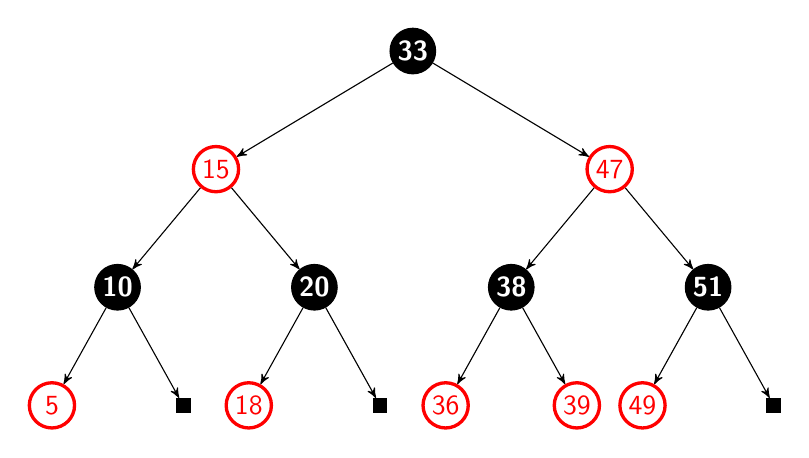
\begin{tikzpicture}[->,>=stealth',level/.style={sibling distance = 5cm/#1,
  level distance = 1.5cm}] 
\node [arn_n] {33}
    child{ node [arn_r] {15} 
            child{ node [arn_n] {10} 
            	child{ node [arn_r] {5}} %for a named pointer
							child{ node [arn_x] {}}
            }
            child{ node [arn_n] {20}
							child{ node [arn_r] {18}}
							child{ node [arn_x] {}}
            }                            
    }
    child{ node [arn_r] {47}
            child{ node [arn_n] {38} 
							child{ node [arn_r] {36}}
							child{ node [arn_r] {39}}
            }
            child{ node [arn_n] {51}
							child{ node [arn_r] {49}}
							child{ node [arn_x] {}}
            }
		}
; 
\end{tikzpicture}
\end{center}


\begin{enumerate}
	\item Its a Height Balanced Binary Search Tree
	\item Every Node is either Red or Black
	\item Root of a Tree is Black
	\item null is also Black
	\item Number of Blacks on Path from root to leaf are same
	\item No Two Consecutive Red, Parent and Children 
	\item Newly Inserted node is Red
	\item Height is $ \Rightarrow \:\: \log{(n)} \leq h \leq 2 \log{(n)}$
\end{enumerate}



\section{Red-Black Tree Creation}

keys : 10, 20, 30, 50, 40, 60, 70, 80, 4, 8


\begin{tcolorbox}
Insertion in Red-Black Tree is just like Binary Search Tree
\end{tcolorbox}

\begin{tcolorbox}
When Inserting New Node the New Node is Red Node
\end{tcolorbox}





\begin{center}
  \bgroup
  \def\arraystretch{1.5}%
  \begin{tabular}{ D C D C  }
  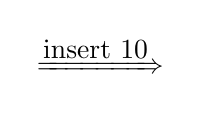
\begin{tikzpicture}
    \draw (0,0) node (arrow) 
{$\xRightarrow{\text{\normalsize insert 10}}$};
    \end{tikzpicture} 
  &
    
\begin{tikzpicture}[->,>=stealth',level/.style={sibling distance = 5cm/#1,
  level distance = 1.5cm}] 
\node [arn_r] {10};
\end{tikzpicture}
    &
    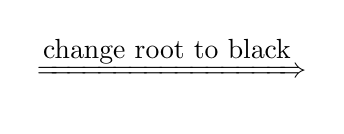
\begin{tikzpicture}
    \draw (0,0) node (arrow) 
{$\xRightarrow{\text{\normalsize change root to black}}$};
    \end{tikzpicture} 
    &
    
\begin{tikzpicture}[->,>=stealth',level/.style={sibling distance = 5cm/#1,
  level distance = 1.5cm}] 
\node [arn_n] {10};
\end{tikzpicture}
     \\ 
  \end{tabular}
  \egroup
\end{center}






\begin{center}
  \bgroup
  \def\arraystretch{1.5}%
  \begin{tabular}{ D C D C  }
    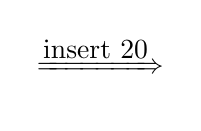
\begin{tikzpicture}
    \draw (0,0) node (arrow) 
{$\xRightarrow{\text{\normalsize insert 20}}$};
    \end{tikzpicture} 
    &
    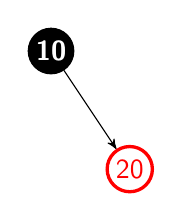
\begin{tikzpicture}[->,>=stealth',level/.style={sibling distance = 2cm,
  level distance = 1.5cm}] 
\node [arn_n] {10}
child [missing] {}
child{
	node [arn_r] {20}
} 
;
\end{tikzpicture}
    &
    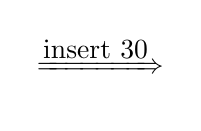
\begin{tikzpicture}
    \draw (0,0) node (arrow) 
{$\xRightarrow{\text{\normalsize insert 30}}$};
    \end{tikzpicture} 
    &
    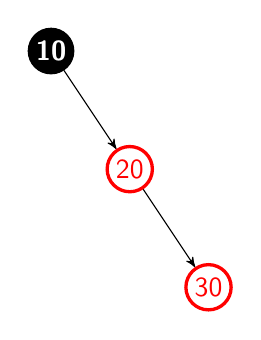
\begin{tikzpicture}[->,>=stealth',level/.style={sibling distance = 2cm,
  level distance = 1.5cm}] 
\node [arn_n] {10}
child [missing] {}
child{
	node [arn_r] {20}
	child [missing] {}
	child{
		node [arn_r] {30}
	} 
} 
;
\end{tikzpicture}
     \\ 
  \end{tabular}
  \egroup
\end{center}




\begin{tcolorbox}
red-red conflict

\noindent
Whenever There is red-red conflict Then you have to do some adjustment for Making It As a Balanced Red-Black Tree .

\noindent
There are Two Approach for Adjustments 
\begin{align*}
\Rightarrow
\begin{cases}
1. Re-Coloring \\
2. Rotation
\end{cases}
\end{align*}
\end{tcolorbox}



When We Have Red-Red conflict It Can Be Two Situation with the Uncle Of That Newly inserted Node


\subsection{Uncle is Red}

\begin{center}
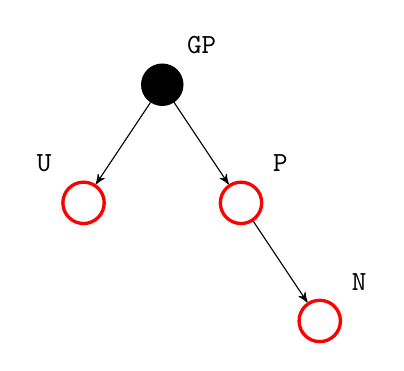
\begin{tikzpicture}[->,>=stealth',level/.style={sibling distance = 2cm,
  level distance = 1.5cm}] 
\node [arn_n] (g) {}
child  {
	node [arn_r] (u) {}
}
child{
	node [arn_r] (p) {}
	child [missing] {}
	child{
		node [arn_r] (n) {}
	} 
} 
;
\node at (g) [xshift=0.5cm,yshift=0.5cm] {\normalsize\ttfamily GP};
\node at (p) [xshift=0.5cm,yshift=0.5cm] {\normalsize\ttfamily P};
\node at (u) [xshift=-0.5cm,yshift=0.5cm] {\normalsize\ttfamily U};
\node at (n) [xshift=0.5cm,yshift=0.5cm] {\normalsize\ttfamily N};
\end{tikzpicture}
\end{center}


When Uncle is Red We Re-Color


\begin{center}
  \bgroup
  \def\arraystretch{1.5}%
  \begin{tabular}{ D D C D  }
    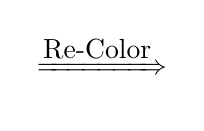
\begin{tikzpicture}
    \draw (0,0) node (arrow) 
{$\xRightarrow{\text{\normalsize Re-Color}}$};
    \end{tikzpicture} 
    &
    &
    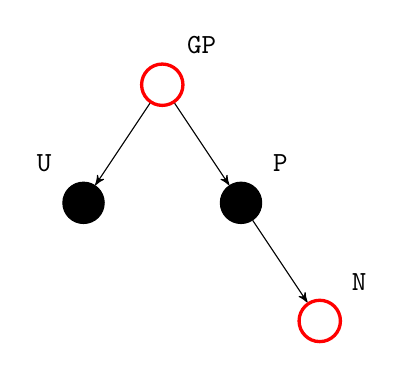
\begin{tikzpicture}[->,>=stealth',level/.style={sibling distance = 2cm,
  level distance = 1.5cm}] 
\node [arn_r] (g) {}
child  {
	node [arn_n] (u) {}
}
child{
	node [arn_n] (p) {}
	child [missing] {}
	child{
		node [arn_r] (n) {}
	} 
} ;
\node at (g) [xshift=0.5cm,yshift=0.5cm] {\normalsize\ttfamily GP};
\node at (p) [xshift=0.5cm,yshift=0.5cm] {\normalsize\ttfamily P};
\node at (u) [xshift=-0.5cm,yshift=0.5cm] {\normalsize\ttfamily U};
\node at (n) [xshift=0.5cm,yshift=0.5cm] {\normalsize\ttfamily N};
\end{tikzpicture}

    &
    
     \\ 
  \end{tabular}
  \egroup
\end{center}


\begin{center}
\begin{lstlisting}[language=C++]
if ( GP == root ) {
	Re-Color GP to Black
}
\end{lstlisting}
\end{center}




\begin{center}
  \bgroup
  \def\arraystretch{1.5}%
  \begin{tabular}{ D D C D  }
    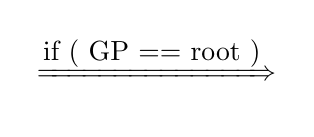
\begin{tikzpicture}
    \draw (0,0) node (arrow) 
{$\xRightarrow{\text{\normalsize if ( GP == root )}}$};
    \end{tikzpicture} 
    &
    &
    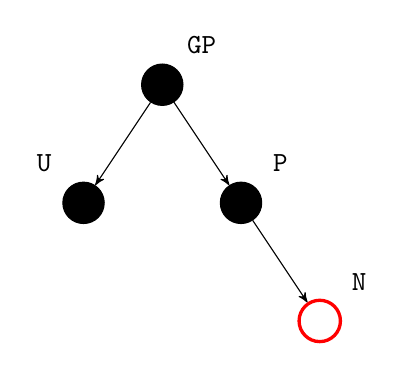
\begin{tikzpicture}[->,>=stealth',level/.style={sibling distance = 2cm,
  level distance = 1.5cm}] 
\node [arn_n] (g) {}
child  {
	node [arn_n] (u) {}
}
child{
	node [arn_n] (p) {}
	child [missing] {}
	child{
		node [arn_r] (n) {}
	} 
} ;
\node at (g) [xshift=0.5cm,yshift=0.5cm] {\normalsize\ttfamily GP};
\node at (p) [xshift=0.5cm,yshift=0.5cm] {\normalsize\ttfamily P};
\node at (u) [xshift=-0.5cm,yshift=0.5cm] {\normalsize\ttfamily U};
\node at (n) [xshift=0.5cm,yshift=0.5cm] {\normalsize\ttfamily N};
\end{tikzpicture}
    
    &
    
     \\ 
  \end{tabular}
  \egroup
\end{center}




\subsection{Uncle is Black}


\begin{center}
  \bgroup
  \def\arraystretch{1.5}%
  \begin{tabular}{ D C C  }
    &
    	Zig-Zig
    &
    Zig-Zag
    \\ \hline
    \\
    &
    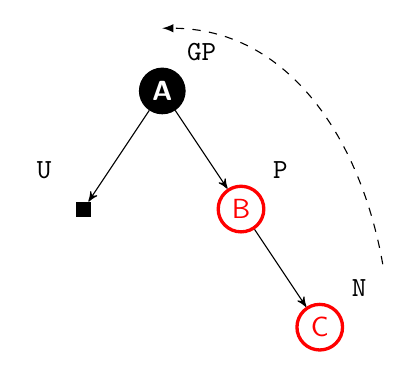
\begin{tikzpicture}[->,>=stealth',level/.style={sibling distance = 2cm,
  level distance = 1.5cm}] 
\node [arn_n] (g) {A}
child  {
	node [arn_x] (u) {}
}
child{
	node [arn_r] (p) {B}
	child [missing] {}
	child{
		node [arn_r] (n) {C}
	} 
} 
;
\node at (g) [xshift=0.5cm,yshift=0.5cm] {\normalsize\ttfamily GP};
\node at (p) [xshift=0.5cm,yshift=0.5cm] {\normalsize\ttfamily P};
\node at (u) [xshift=-0.5cm,yshift=0.5cm] {\normalsize\ttfamily U};
\node at (n) [xshift=0.5cm,yshift=0.5cm] {\normalsize\ttfamily N};

\coordinate (A) at ([yshift=.8cm,xshift=0.8cm]n);
%\coordinate (C) at ([yshift=.5cm,xshift=1cm]r);
\coordinate (C) at ([yshift=.5cm]g.north);

%\draw[dashed] plot[smooth] coordinates {(C) (A)};
\draw[->,>=latex,dashed] (A) to[out=100,in=0] (C);
\end{tikzpicture}
    &
      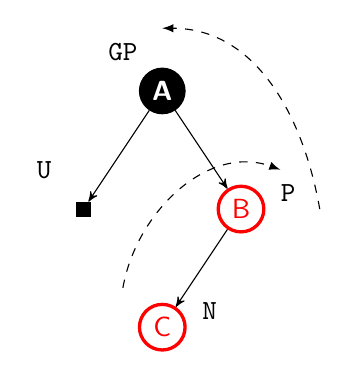
\begin{tikzpicture}[->,>=stealth',level/.style={sibling distance = 2cm,
  level distance = 1.5cm}] 
\node [arn_n] (g) {A}
child  {
	node [arn_x] (u) {}
}
child{
	node [arn_r] (p) {B}
	child{
		node [arn_r] (n) {C}
	} 
	child [missing] {}
} 
;
\node at (g) [xshift=-0.5cm,yshift=0.5cm] {\normalsize\ttfamily GP};
\node at (p) [xshift=0.6cm,yshift=0.2cm] {\normalsize\ttfamily P};
\node at (u) [xshift=-0.5cm,yshift=0.5cm] {\normalsize\ttfamily U};
\node at (n) [xshift=0.6cm,yshift=0.2cm] {\normalsize\ttfamily N};

\coordinate (A) at ([xshift=1cm]p);
\coordinate (C) at ([yshift=.5cm]g.north);

\coordinate (E) at ([yshift=0.5cm,xshift=-0.5cm]n);
%\coordinate (F) at ([yshift=.5cm]a);
\coordinate (G) at ([xshift=0.5cm,yshift=0.5cm]p);

%\draw[dashed] plot[smooth] coordinates {(C) (A)};
\draw[->,>=latex,dashed] (A) to[out=100,in=0] (C);
\draw[->,>=latex,dashed] (E) to[out=80,in=160] (G) ;
\end{tikzpicture}
     \\ 
     \\
     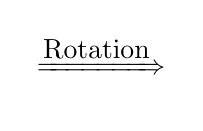
\begin{tikzpicture}
    \draw (0,0) node (arrow) 
{$\xRightarrow{\text{\normalsize Rotation}}$};
    \end{tikzpicture} 
     &
      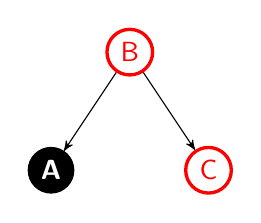
\begin{tikzpicture}[->,>=stealth',level/.style={sibling distance = 2cm,
  level distance = 1.5cm}] 
\node [arn_r] (g) {B}
child  {
	node [arn_n] {A}
}
child{
	node [arn_r] {C}
} 
;
\end{tikzpicture}
    &
	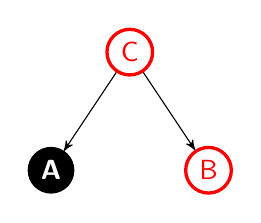
\begin{tikzpicture}[->,>=stealth',level/.style={sibling distance = 2cm,
	  level distance = 1.5cm}] 
	\node [arn_r] (g) {C}
	child  {
		node [arn_n] {A}
	}
	child{
		node [arn_r] {B}
	} 
	;
	\end{tikzpicture}
     \\ 
     \\
     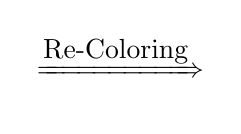
\begin{tikzpicture}
    \draw (0,0) node (arrow) 
{$\xRightarrow{\text{\normalsize Re-Coloring}}$};
    \end{tikzpicture} 
     &
      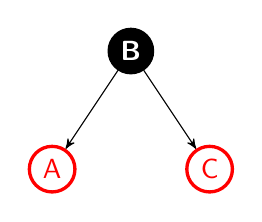
\begin{tikzpicture}[->,>=stealth',level/.style={sibling distance = 2cm,
  level distance = 1.5cm}] 
\node [arn_n] (g) {B}
child  {
	node [arn_r] {A}
}
child{
	node [arn_r] {C}
} 
;
\end{tikzpicture}
    &
	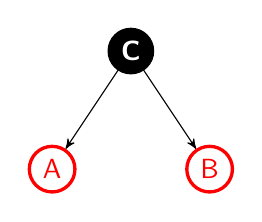
\begin{tikzpicture}[->,>=stealth',level/.style={sibling distance = 2cm,
	  level distance = 1.5cm}] 
	\node [arn_n] (g) {C}
	child  {
		node [arn_r] {A}
	}
	child{
		node [arn_r] {B}
	} 
	;
	\end{tikzpicture}
  \end{tabular}
  \egroup
\end{center}










\begin{center}
  \bgroup
  \def\arraystretch{1.5}%
  \begin{tabular}{ D C C  }
    &
    	Zig-Zig
    &
    Zig-Zag
    \\ \hline
    \\
    &
    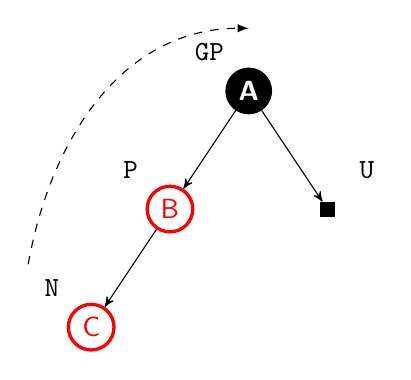
\begin{tikzpicture}[->,>=stealth',level/.style={sibling distance = 2cm,
  level distance = 1.5cm}] 
\node [arn_n] (g) {A}
child{
	node [arn_r] (p) {B}
	child{
		node [arn_r] (n) {C}
	} 
	child [missing] {}
} 
child  {
	node [arn_x] (u) {}
}
;
\node at (g) [xshift=-0.5cm,yshift=0.5cm] {\normalsize\ttfamily GP};
\node at (p) [xshift=-0.5cm,yshift=0.5cm] {\normalsize\ttfamily P};
\node at (u) [xshift=0.5cm,yshift=0.5cm] {\normalsize\ttfamily U};
\node at (n) [xshift=-0.5cm,yshift=0.5cm] {\normalsize\ttfamily N};

\coordinate (A) at ([yshift=.8cm,xshift=-0.8cm]n);
%\coordinate (C) at ([yshift=.5cm,xshift=1cm]r);
\coordinate (C) at ([yshift=.5cm]g.north);

%\draw[dashed] plot[smooth] coordinates {(C) (A)};
\draw[->,>=latex,dashed] (A) to[out=80,in=180] (C);
\end{tikzpicture}
    &
      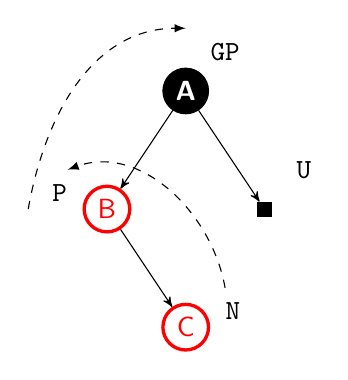
\begin{tikzpicture}[->,>=stealth',level/.style={sibling distance = 2cm,
  level distance = 1.5cm}] 
\node [arn_n] (g) {A}
child{
	node [arn_r] (p) {B}
	child [missing] {}
	child{
		node [arn_r] (n) {C}
	} 
} 
child  {
	node [arn_x] (u) {}
}
;
\node at (g) [xshift=0.5cm,yshift=0.5cm] {\normalsize\ttfamily GP};
\node at (p) [xshift=-0.6cm,yshift=0.2cm] {\normalsize\ttfamily P};
\node at (u) [xshift=0.5cm,yshift=0.5cm] {\normalsize\ttfamily U};
\node at (n) [xshift=0.6cm,yshift=0.2cm] {\normalsize\ttfamily N};

\coordinate (A) at ([xshift=-1cm]p);
\coordinate (C) at ([yshift=.5cm]g.north);

\coordinate (E) at ([yshift=0.5cm,xshift=0.5cm]n);
%\coordinate (F) at ([yshift=.5cm]a);
\coordinate (G) at ([xshift=-0.5cm,yshift=0.5cm]p);

%\draw[dashed] plot[smooth] coordinates {(C) (A)};
\draw[->,>=latex,dashed] (A) to[out=80,in=180] (C);
\draw[->,>=latex,dashed] (E) to[out=100,in=20] (G) ;
\end{tikzpicture}
     \\ 
     \\
     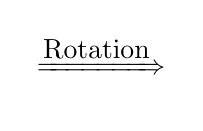
\begin{tikzpicture}
    \draw (0,0) node (arrow) 
{$\xRightarrow{\text{\normalsize Rotation}}$};
    \end{tikzpicture} 
     &
      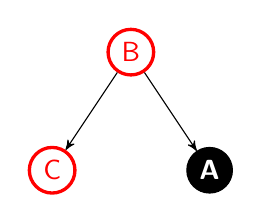
\begin{tikzpicture}[->,>=stealth',level/.style={sibling distance = 2cm,
  level distance = 1.5cm}] 
\node [arn_r] (g) {B}
child  {
	node [arn_r] {C}
}
child{
	node [arn_n] {A}
} 
;
\end{tikzpicture}
    &
	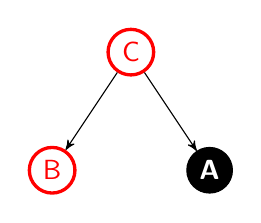
\begin{tikzpicture}[->,>=stealth',level/.style={sibling distance = 2cm,
	  level distance = 1.5cm}] 
	\node [arn_r] (g) {C}
	child  {
		node [arn_r] {B}
	}
	child{
		node [arn_n] {A}
	} 
	;
	\end{tikzpicture}
     \\ 
     \\
     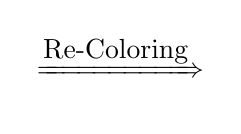
\begin{tikzpicture}
    \draw (0,0) node (arrow) 
{$\xRightarrow{\text{\normalsize Re-Coloring}}$};
    \end{tikzpicture} 
     &
      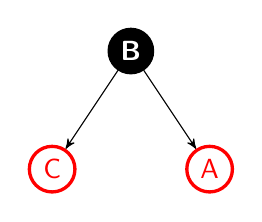
\begin{tikzpicture}[->,>=stealth',level/.style={sibling distance = 2cm,
  level distance = 1.5cm}] 
\node [arn_n] (g) {B}
child  {
	node [arn_r] {C}
}
child{
	node [arn_r] {A}
} 
;
\end{tikzpicture}
    &
	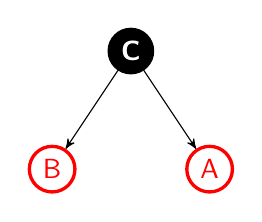
\begin{tikzpicture}[->,>=stealth',level/.style={sibling distance = 2cm,
	  level distance = 1.5cm}] 
	\node [arn_n] (g) {C}
	child  {
		node [arn_r] {B}
	}
	child{
		node [arn_r] {A}
	} 
	;
	\end{tikzpicture}
  \end{tabular}
  \egroup
\end{center}



now we continue our Red-Black Tree Creation :



\begin{center}
  \bgroup
  \def\arraystretch{1.5}%
  \begin{tabular}{ D C  }
    \begin{tikzpicture}
    \draw (0,0) node (arrow) 
{$\Longrightarrow{\text{\normalsize}}$};
    \end{tikzpicture} 
    &
    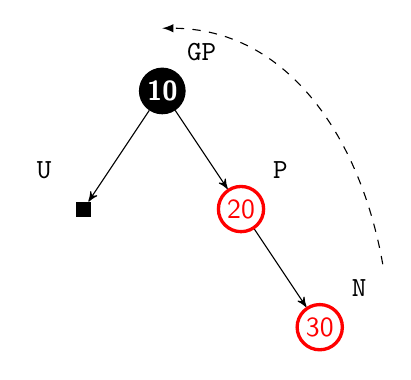
\begin{tikzpicture}[->,>=stealth',level/.style={sibling distance = 2cm,
  level distance = 1.5cm}] 
\node [arn_n] (g) {10}
child  {
	node [arn_x] (u) {}
}
child{
	node [arn_r] (p) {20}
	child [missing] {}
	child{
		node [arn_r] (n) {30}
	} 
};
\node at (g) [xshift=0.5cm,yshift=0.5cm] {\normalsize\ttfamily GP};
\node at (p) [xshift=0.5cm,yshift=0.5cm] {\normalsize\ttfamily P};
\node at (u) [xshift=-0.5cm,yshift=0.5cm] {\normalsize\ttfamily U};
\node at (n) [xshift=0.5cm,yshift=0.5cm] {\normalsize\ttfamily N};

\coordinate (A) at ([yshift=.8cm,xshift=0.8cm]n);
%\coordinate (C) at ([yshift=.5cm,xshift=1cm]r);
\coordinate (C) at ([yshift=.5cm]g.north);

%\draw[dashed] plot[smooth] coordinates {(C) (A)};
\draw[->,>=latex,dashed] (A) to[out=100,in=0] (C);
\end{tikzpicture}
     \\ 
  \end{tabular}
  \egroup
\end{center}






\begin{center}
  \bgroup
  \def\arraystretch{1.5}%
  \begin{tabular}{ D C D C  }
     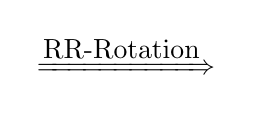
\begin{tikzpicture}
    \draw (0,0) node (arrow) 
{$\xRightarrow{\text{\normalsize RR-Rotation}}$};
    \end{tikzpicture} 
     &
      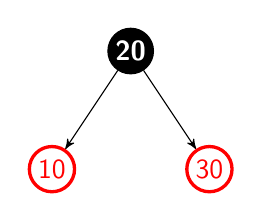
\begin{tikzpicture}[->,>=stealth',level/.style={sibling distance = 2cm,
  level distance = 1.5cm}] 
\node [arn_n] (g) {20}
child  {
	node [arn_r] {10}
}
child{
	node [arn_r] {30}
} 
;
\end{tikzpicture}
     \\ 
  \end{tabular}
  \egroup
\end{center}









\begin{center}
  \bgroup
  \def\arraystretch{1.5}%
  \begin{tabular}{ D C D C  }
     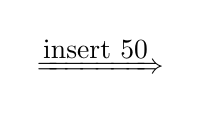
\begin{tikzpicture}
    \draw (0,0) node (arrow) 
{$\xRightarrow{\text{\normalsize insert 50}}$};
    \end{tikzpicture} 
     &
      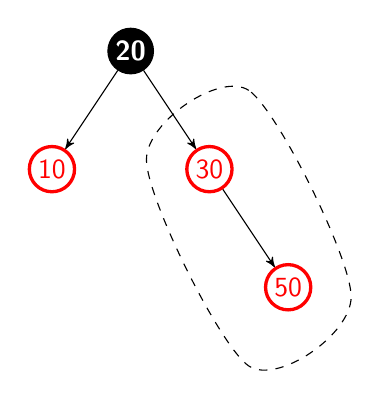
\begin{tikzpicture}[->,>=stealth',level/.style={sibling distance = 2cm,
  level distance = 1.5cm}] 
\node [arn_n] (g) {20}
child  {
	node [arn_r] (u) {10}
}
child{
	node [arn_r] (p) {30}
	child [missing] {}
	child{
	    node [arn_r] (n) {50}
    } 
};
%\node at (g) [xshift=0.5cm,yshift=0.5cm] {\normalsize\ttfamily GP};
%\node at (p) [xshift=0.5cm,yshift=0.5cm] {\normalsize\ttfamily P};
%\node at (u) [xshift=-0.5cm,yshift=0.5cm] {\normalsize\ttfamily U};
%\node at (n) [xshift=0.5cm,yshift=0.5cm] {\normalsize\ttfamily N};

\coordinate (A) at ([yshift=-0.12cm,xshift=0.8cm]n);
\coordinate (AA) at ([yshift=-1cm,xshift=-0.5cm]n);
%\coordinate (C) at ([yshift=.5cm,xshift=1cm]r);
\coordinate (C) at ([yshift=.5cm]g.north);

\coordinate (B) at ([yshift=1cm,xshift=0.5cm]p);
\coordinate (BB) at ([yshift=0.12cm,xshift=-0.8cm]p);

\draw[dashed] plot[smooth cycle] coordinates {(A) (B) (BB)  (AA)};
%\draw[->,>=latex,dashed] (A) to[out=100,in=0] (C);
\end{tikzpicture}
     \\ 
  \end{tabular}
  \egroup
\end{center}



\begin{tcolorbox}
\begin{itemize}
	\item Red-Red Conflict
	\item Uncle is red $\to$ Re-Coloring
\end{itemize}
\end{tcolorbox}






\begin{center}
  \bgroup
  \def\arraystretch{1.5}%
  \begin{tabular}{ D C D C  }
     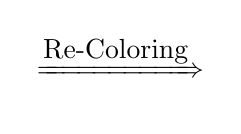
\begin{tikzpicture}
    \draw (0,0) node (arrow) 
{$\xRightarrow{\text{\normalsize Re-Coloring}}$};
    \end{tikzpicture} 
     &
      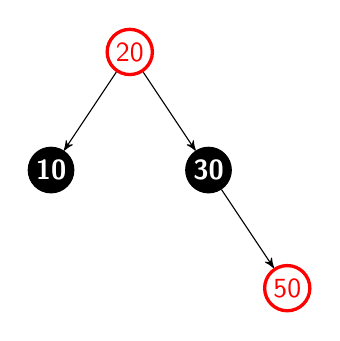
\begin{tikzpicture}[->,>=stealth',level/.style={sibling distance = 2cm,
  level distance = 1.5cm}] 
\node [arn_r] (g) {20}
child  {
	node [arn_n] (u) {10}
}
child{
	node [arn_n] (p) {30}
	child [missing] {}
	child{
	    node [arn_r] (n) {50}
    } 
};
%\node at (g) [xshift=0.5cm,yshift=0.5cm] {\normalsize\ttfamily GP};
%\node at (p) [xshift=0.5cm,yshift=0.5cm] {\normalsize\ttfamily P};
%\node at (u) [xshift=-0.5cm,yshift=0.5cm] {\normalsize\ttfamily U};
%\node at (n) [xshift=0.5cm,yshift=0.5cm] {\normalsize\ttfamily N};

%\coordinate (A) at ([yshift=-0.12cm,xshift=0.8cm]n);
%\coordinate (AA) at ([yshift=-1cm,xshift=-0.5cm]n);
%\coordinate (C) at ([yshift=.5cm,xshift=1cm]r);
%\coordinate (C) at ([yshift=.5cm]g.north);

%\coordinate (B) at ([yshift=1cm,xshift=0.5cm]p);
%\coordinate (BB) at ([yshift=0.12cm,xshift=-0.8cm]p);

%\draw[dashed] plot[smooth cycle] coordinates {(A) (B) (BB)  (AA)};
%\draw[->,>=latex,dashed] (A) to[out=100,in=0] (C);
\end{tikzpicture}
     \\ 
  \end{tabular}
  \egroup
\end{center}


\begin{center}
\begin{lstlisting}[language=C++]
if ( GP == root ) {
	Re-Color GP to Black
}
\end{lstlisting}
\end{center}









\begin{center}
  \bgroup
  \def\arraystretch{1.5}%
  \begin{tabular}{ C C  }
     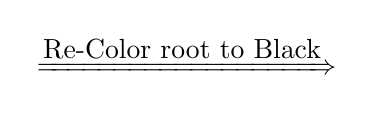
\begin{tikzpicture}
    \draw (0,0) node (arrow) 
{$\xRightarrow{\text{\normalsize Re-Color root to Black}}$};
    \end{tikzpicture} 
     &
      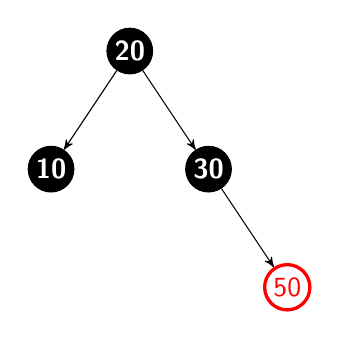
\begin{tikzpicture}[->,>=stealth',level/.style={sibling distance = 2cm,
  level distance = 1.5cm}] 
\node [arn_n] (g) {20}
child  {
	node [arn_n] (u) {10}
}
child{
	node [arn_n] (p) {30}
	child [missing] {}
	child{
	    node [arn_r] (n) {50}
    } 
};
%\node at (g) [xshift=0.5cm,yshift=0.5cm] {\normalsize\ttfamily GP};
%\node at (p) [xshift=0.5cm,yshift=0.5cm] {\normalsize\ttfamily P};
%\node at (u) [xshift=-0.5cm,yshift=0.5cm] {\normalsize\ttfamily U};
%\node at (n) [xshift=0.5cm,yshift=0.5cm] {\normalsize\ttfamily N};

%\coordinate (A) at ([yshift=-0.12cm,xshift=0.8cm]n);
%\coordinate (AA) at ([yshift=-1cm,xshift=-0.5cm]n);
%\coordinate (C) at ([yshift=.5cm,xshift=1cm]r);
%\coordinate (C) at ([yshift=.5cm]g.north);

%\coordinate (B) at ([yshift=1cm,xshift=0.5cm]p);
%\coordinate (BB) at ([yshift=0.12cm,xshift=-0.8cm]p);

%\draw[dashed] plot[smooth cycle] coordinates {(A) (B) (BB)  (AA)};
%\draw[->,>=latex,dashed] (A) to[out=100,in=0] (C);
\end{tikzpicture}
     \\ 
  \end{tabular}
  \egroup
\end{center}









\begin{center}
  \bgroup
  \def\arraystretch{1.5}%
  \begin{tabular}{ C C  }
     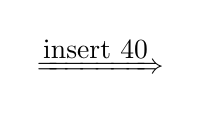
\begin{tikzpicture}
    \draw (0,0) node (arrow) 
{$\xRightarrow{\text{\normalsize insert 40}}$};
    \end{tikzpicture} 
     &
      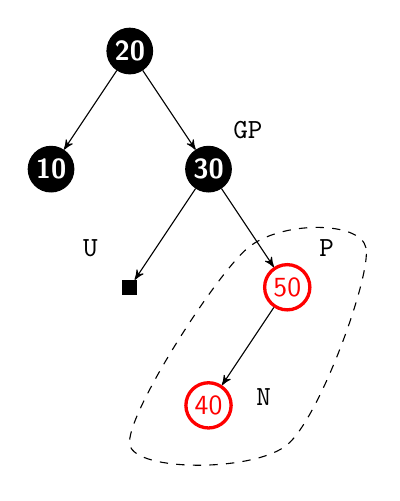
\begin{tikzpicture}[->,>=stealth',level/.style={sibling distance = 2cm,
  level distance = 1.5cm}] 
\node [arn_n]  {20}
child  {
	node [arn_n]  {10}
}
child{
	node [arn_n] (g) {30}
	child {
	    node [arn_x] (u) {}
	}
	child{
	    node [arn_r] (p) {50}
	    child{
	       node [arn_r] (n) {40}
	    } child [missing] {}
    } 
};
\node at (g) [xshift=0.5cm,yshift=0.5cm] {\normalsize\ttfamily GP};
\node at (p) [xshift=0.5cm,yshift=0.5cm] {\normalsize\ttfamily P};
\node at (u) [xshift=-0.5cm,yshift=0.5cm] {\normalsize\ttfamily U};
\node at (n) [xshift=0.7cm,yshift=0.1cm] {\normalsize\ttfamily N};

\coordinate (A) at ([yshift=-0.5cm,xshift=1cm]n);
\coordinate (AA) at ([yshift=-0.5cm,xshift=-1cm]n);
%\coordinate (C) at ([yshift=.5cm,xshift=1cm]r);
%\coordinate (C) at ([yshift=.5cm]g.north);

\coordinate (B) at ([yshift=0.5cm,xshift=1cm]p);
\coordinate (BB) at ([yshift=0.5cm,xshift=-0.5cm]p);

\draw[dashed] plot[smooth cycle] coordinates {(A) (B) (BB)  (AA)};
%\draw[->,>=latex,dashed] (A) to[out=100,in=0] (C);
\end{tikzpicture}
     \\ 
  \end{tabular}
  \egroup
\end{center}



\begin{tcolorbox}
\begin{itemize}
	\item Red-Red Conflict
	\item Uncle is Black $\to$ Perform Rotation
\end{itemize}
\end{tcolorbox}






\begin{center}
  \bgroup
  \def\arraystretch{1.5}%
  \begin{tabular}{ C C  }
     \begin{tikzpicture}
    \draw (0,0) node (arrow) 
{$\Longrightarrow{\text{\normalsize}}$};
    \end{tikzpicture} 
     &
      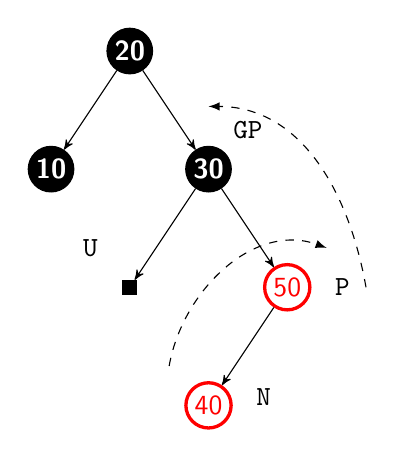
\begin{tikzpicture}[->,>=stealth',level/.style={sibling distance = 2cm,
  level distance = 1.5cm}] 
\node [arn_n]  {20}
child  {
	node [arn_n]  {10}
}
child{
	node [arn_n] (g) {30}
	child {
	    node [arn_x] (u) {}
	}
	child{
	    node [arn_r] (p) {50}
	    child{
	       node [arn_r] (n) {40}
	    } child [missing] {}
    } 
};
\node at (g) [xshift=0.5cm,yshift=0.5cm] {\normalsize\ttfamily GP};
\node at (p) [xshift=0.7cm,yshift=0cm] {\normalsize\ttfamily P};
\node at (u) [xshift=-0.5cm,yshift=0.5cm] {\normalsize\ttfamily U};
\node at (n) [xshift=0.7cm,yshift=0.1cm] {\normalsize\ttfamily N};

%\coordinate (A) at ([yshift=-0.5cm,xshift=1cm]n);
%\coordinate (AA) at ([yshift=-0.5cm,xshift=-1cm]n);
%\coordinate (C) at ([yshift=.5cm,xshift=1cm]r);
%\coordinate (C) at ([yshift=.5cm]g.north);

%\coordinate (B) at ([yshift=0.5cm,xshift=1cm]p);
%\coordinate (BB) at ([yshift=0.5cm,xshift=-0.5cm]p);

%\draw[dashed] plot[smooth cycle] coordinates {(A) (B) (BB)  (AA)};
%\draw[->,>=latex,dashed] (A) to[out=100,in=0] (C);
\coordinate (A) at ([xshift=1cm]p);
\coordinate (C) at ([yshift=.5cm]g.north);

\coordinate (E) at ([yshift=0.5cm,xshift=-0.5cm]n);
%\coordinate (F) at ([yshift=.5cm]a);
\coordinate (G) at ([xshift=0.5cm,yshift=0.5cm]p);

%\draw[dashed] plot[smooth] coordinates {(C) (A)};
\draw[->,>=latex,dashed] (A) to[out=100,in=0] (C);
\draw[->,>=latex,dashed] (E) to[out=80,in=160] (G) ;
\end{tikzpicture}
     \\ 
  \end{tabular}
  \egroup
\end{center}









\begin{center}
  \bgroup
  \def\arraystretch{1.5}%
  \begin{tabular}{ C C  }
     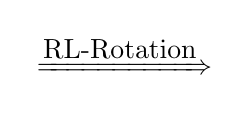
\begin{tikzpicture}
    \draw (0,0) node (arrow) 
{$\xRightarrow{\text{\normalsize RL-Rotation}}$};
    \end{tikzpicture} 
     &
      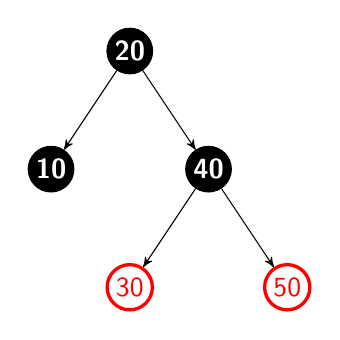
\begin{tikzpicture}[->,>=stealth',level/.style={sibling distance = 2cm,
  level distance = 1.5cm}] 
\node [arn_n] (g) {20}
child  {
	node [arn_n]  {10}
}
child{
    node [arn_n]  {40}
	child {
	    node [arn_r]  {30}
	}
	child{
	    node [arn_r]  {50}
    } 
};
%\node at (g) [xshift=0.5cm,yshift=0.5cm] {\normalsize\ttfamily GP};
%\node at (p) [xshift=0.7cm,yshift=0cm] {\normalsize\ttfamily P};
%\node at (u) [xshift=-0.5cm,yshift=0.5cm] {\normalsize\ttfamily U};
%\node at (n) [xshift=0.7cm,yshift=0.1cm] {\normalsize\ttfamily N};

%\coordinate (A) at ([yshift=-0.5cm,xshift=1cm]n);
%\coordinate (AA) at ([yshift=-0.5cm,xshift=-1cm]n);
%\coordinate (C) at ([yshift=.5cm,xshift=1cm]r);
%\coordinate (C) at ([yshift=.5cm]g.north);

%\coordinate (B) at ([yshift=0.5cm,xshift=1cm]p);
%\coordinate (BB) at ([yshift=0.5cm,xshift=-0.5cm]p);

%\draw[dashed] plot[smooth cycle] coordinates {(A) (B) (BB)  (AA)};
%\draw[->,>=latex,dashed] (A) to[out=100,in=0] (C);
\end{tikzpicture}
     \\ 
  \end{tabular}
  \egroup
\end{center}











\begin{center}
  \bgroup
  \def\arraystretch{1.5}%
  \begin{tabular}{ C C  }
     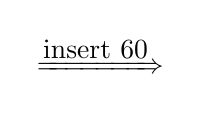
\begin{tikzpicture}
    \draw (0,0) node (arrow) 
{$\xRightarrow{\text{\normalsize insert 60}}$};
    \end{tikzpicture} 
     &
      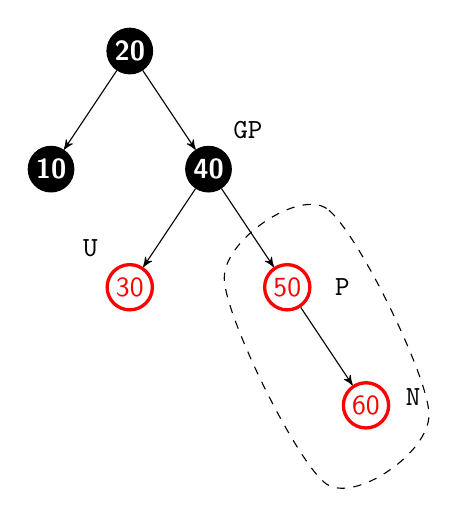
\begin{tikzpicture}[->,>=stealth',level/.style={sibling distance = 2cm,
  level distance = 1.5cm}] 
\node [arn_n] {20}
child  {
	node [arn_n]  {10}
}
child{
    node [arn_n] (g) {40}
	child {
	    node [arn_r] (u) {30}
	}
	child{
	    node [arn_r] (p) {50}
	    child [missing] {}
	    child {
	        node [arn_r] (n) {60}
	    }
    } 
};
\node at (g) [xshift=0.5cm,yshift=0.5cm] {\normalsize\ttfamily GP};
\node at (p) [xshift=0.7cm,yshift=0cm] {\normalsize\ttfamily P};
\node at (u) [xshift=-0.5cm,yshift=0.5cm] {\normalsize\ttfamily U};
\node at (n) [xshift=0.6cm,yshift=0.1cm] {\normalsize\ttfamily N};

\coordinate (A) at ([yshift=-0.12cm,xshift=0.8cm]n);
\coordinate (AA) at ([yshift=-1cm,xshift=-0.5cm]n);
%\coordinate (C) at ([yshift=.5cm,xshift=1cm]r);
\coordinate (C) at ([yshift=.5cm]g.north);

\coordinate (B) at ([yshift=1cm,xshift=0.5cm]p);
\coordinate (BB) at ([yshift=0.12cm,xshift=-0.8cm]p);

\draw[dashed] plot[smooth cycle] coordinates {(A) (B) (BB)  (AA)};
%\draw[->,>=latex,dashed] (A) to[out=100,in=0] (C);
\end{tikzpicture}
     \\ 
  \end{tabular}
  \egroup
\end{center}




\begin{tcolorbox}
\begin{itemize}
	\item Red-Red Conflict
	\item Uncle is red $\to$ Re-Coloring
\end{itemize}
\end{tcolorbox}





\begin{center}
  \bgroup
  \def\arraystretch{1.5}%
  \begin{tabular}{ C C  }
     \begin{tikzpicture}
    \draw (0,0) node (arrow) 
{$\Longrightarrow{\text{\normalsize}}$};
    \end{tikzpicture} 
     &
      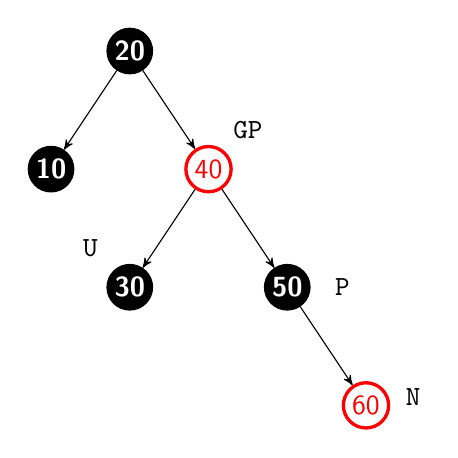
\begin{tikzpicture}[->,>=stealth',level/.style={sibling distance = 2cm,
  level distance = 1.5cm}] 
\node [arn_n]  {20}
child  {
	node [arn_n] {10}
}
child{
    node [arn_r] (g) {40}
	child {
	    node [arn_n] (u) {30}
	}
	child{
	    node [arn_n] (p) {50}
	    child [missing] {}
	    child {
	        node [arn_r] (n) {60}
	    }
    } 
};
\node at (g) [xshift=0.5cm,yshift=0.5cm] {\normalsize\ttfamily GP};
\node at (p) [xshift=0.7cm,yshift=0cm] {\normalsize\ttfamily P};
\node at (u) [xshift=-0.5cm,yshift=0.5cm] {\normalsize\ttfamily U};
\node at (n) [xshift=0.6cm,yshift=0.1cm] {\normalsize\ttfamily N};

%\coordinate (A) at ([yshift=-0.12cm,xshift=0.8cm]n);
%\coordinate (AA) at ([yshift=-1cm,xshift=-0.5cm]n);
%\coordinate (C) at ([yshift=.5cm,xshift=1cm]r);
%\coordinate (C) at ([yshift=.5cm]g.north);

%\coordinate (B) at ([yshift=1cm,xshift=0.5cm]p);
%\coordinate (BB) at ([yshift=0.12cm,xshift=-0.8cm]p);

%\draw[dashed] plot[smooth cycle] coordinates {(A) (B) (BB)  (AA)};
%\draw[->,>=latex,dashed] (A) to[out=100,in=0] (C);
\end{tikzpicture}
     \\ 
  \end{tabular}
  \egroup
\end{center}






\begin{tcolorbox}
\begin{itemize}
	\item Now Again for GP, check It's Ancestor to see there is Red-Red Conflict , You should check this untill There is no conflict
	\item in this case the Ancestor is black and there is no Red-Red conflict, so we don't need to do anything more
\end{itemize}
\end{tcolorbox}














\begin{center}
  \bgroup
  \def\arraystretch{1.5}%
  \begin{tabular}{ C C  }
     \begin{tikzpicture}
    \draw (0,0) node (arrow) 
{$\xRightarrow{\text{\normalsize insert 70}}$};
    \end{tikzpicture} 
     &
      \begin{tikzpicture}[->,>=stealth',level/.style={sibling distance = 2cm,
  level distance = 1.5cm}] 
\node [arn_n]  {20}
child  {
	node [arn_n] {10}
}
child{
    node [arn_r]  {40}
	child {
	    node [arn_n]  {30}
	}
	child{
	    node [arn_n] (g) {50}
	    child  {
	         node [arn_x] (u) {}
	    }
	    child {
	        node [arn_r] (p) {60}
	        child [missing] {}
	        child {
	             node [arn_r] (n) {70}
	        }
	    }
    } 
};
\node at (g) [xshift=0.5cm,yshift=0.5cm] {\normalsize\ttfamily GP};
\node at (p) [xshift=0.7cm,yshift=0cm] {\normalsize\ttfamily P};
\node at (u) [xshift=-0.5cm,yshift=0.5cm] {\normalsize\ttfamily U};
\node at (n) [xshift=0.6cm,yshift=0.1cm] {\normalsize\ttfamily N};

\coordinate (A) at ([yshift=-0.12cm,xshift=0.8cm]n);
\coordinate (AA) at ([yshift=-1cm,xshift=-0.5cm]n);
%\coordinate (C) at ([yshift=.5cm,xshift=1cm]r);
%\coordinate (C) at ([yshift=.5cm]g.north);

\coordinate (B) at ([yshift=1cm,xshift=0.5cm]p);
\coordinate (BB) at ([yshift=0.12cm,xshift=-0.8cm]p);

\draw[dashed] plot[smooth cycle] coordinates {(A) (B) (BB)  (AA)};
%\draw[->,>=latex,dashed] (A) to[out=100,in=0] (C);
\end{tikzpicture}
     \\ 
  \end{tabular}
  \egroup
\end{center}



\begin{tcolorbox}
\begin{itemize}
	\item Red-Red Conflict
	\item Uncle is black $\to$ Rotation
\end{itemize}
\end{tcolorbox}







\begin{center}
  \bgroup
  \def\arraystretch{1.5}%
  \begin{tabular}{ C C  }
     \begin{tikzpicture}
    \draw (0,0) node (arrow) 
{$\Longrightarrow{\text{\normalsize}}$};
    \end{tikzpicture} 
     &
      \begin{tikzpicture}[->,>=stealth',level/.style={sibling distance = 2cm,
  level distance = 1.5cm}] 
\node [arn_n]  {20}
child  {
	node [arn_n] {10}
}
child{
    node [arn_r]  {40}
	child {
	    node [arn_n]  {30}
	}
	child{
	    node [arn_n] (g) {50}
	    child  {
	         node [arn_x] (u) {}
	    }
	    child {
	        node [arn_r] (p) {60}
	        child [missing] {}
	        child {
	             node [arn_r] (n) {70}
	        }
	    }
    } 
};
\node at (g) [xshift=0.5cm,yshift=0.5cm] {\normalsize\ttfamily GP};
\node at (p) [xshift=0.7cm,yshift=0cm] {\normalsize\ttfamily P};
\node at (u) [xshift=-0.5cm,yshift=0.5cm] {\normalsize\ttfamily U};
\node at (n) [xshift=0.6cm,yshift=0.1cm] {\normalsize\ttfamily N};

%\coordinate (A) at ([yshift=-0.12cm,xshift=0.8cm]n);
%\coordinate (AA) at ([yshift=-1cm,xshift=-0.5cm]n);
%\coordinate (C) at ([yshift=.5cm,xshift=1cm]r);
%\coordinate (C) at ([yshift=.5cm]g.north);

%\coordinate (B) at ([yshift=1cm,xshift=0.5cm]p);
%\coordinate (BB) at ([yshift=0.12cm,xshift=-0.8cm]p);

%\draw[dashed] plot[smooth cycle] coordinates {(A) (B) (BB)  (AA)};
%\draw[->,>=latex,dashed] (A) to[out=100,in=0] (C);
\coordinate (A) at ([yshift=.8cm,xshift=0.8cm]n);
%\coordinate (C) at ([yshift=.5cm,xshift=1cm]r);
\coordinate (C) at ([yshift=.5cm]g.north);

%\draw[dashed] plot[smooth] coordinates {(C) (A)};
\draw[->,>=latex,dashed] (A) to[out=100,in=0] (C);
\end{tikzpicture}
     \\ 
  \end{tabular}
  \egroup
\end{center}









\begin{center}
  \bgroup
  \def\arraystretch{1.5}%
  \begin{tabular}{ C C  }
     \begin{tikzpicture}
    \draw (0,0) node (arrow) 
{$\xRightarrow{\text{\normalsize RR-Rotation}}$};
    \end{tikzpicture} 
     &
      \begin{tikzpicture}[->,>=stealth',level/.style={sibling distance = 2cm,
  level distance = 1.5cm}] 
\node [arn_n]  {20}
child  {
	node [arn_n] {10}
}
child{
    node [arn_r]  {40}
	child {
	    node [arn_n]  {30}
	}
	child{
	     node [arn_n] (p) {60}
	        child {
	             node [arn_r] (g) {50}
	        }
	        child {
	             node [arn_r] (n) {70}
	        }
    } 
};
%\node at (g) [xshift=0.5cm,yshift=0.5cm] {\normalsize\ttfamily GP};
%\node at (p) [xshift=0.7cm,yshift=0cm] {\normalsize\ttfamily P};
%\node at (u) [xshift=-0.5cm,yshift=0.5cm] {\normalsize\ttfamily U};
%\node at (n) [xshift=0.6cm,yshift=0.1cm] {\normalsize\ttfamily N};

%\coordinate (A) at ([yshift=-0.12cm,xshift=0.8cm]n);
%\coordinate (AA) at ([yshift=-1cm,xshift=-0.5cm]n);
%\coordinate (C) at ([yshift=.5cm,xshift=1cm]r);
%\coordinate (C) at ([yshift=.5cm]g.north);

%\coordinate (B) at ([yshift=1cm,xshift=0.5cm]p);
%\coordinate (BB) at ([yshift=0.12cm,xshift=-0.8cm]p);

%\draw[dashed] plot[smooth cycle] coordinates {(A) (B) (BB)  (AA)};
%\draw[->,>=latex,dashed] (A) to[out=100,in=0] (C);
\end{tikzpicture}
     \\ 
  \end{tabular}
  \egroup
\end{center}











\begin{center}
  \bgroup
  \def\arraystretch{1.5}%
  \begin{tabular}{ C C  }
     \begin{tikzpicture}
    \draw (0,0) node (arrow) 
{$\xRightarrow{\text{\normalsize insert 80}}$};
    \end{tikzpicture} 
     &
      \begin{tikzpicture}[->,>=stealth',level/.style={sibling distance = 2cm,
  level distance = 1.5cm}] 
\node [arn_n]  {20}
child  {
	node [arn_n] {10}
}
child{
    node [arn_r]  {40}
	child {
	    node [arn_n]  {30}
	}
	child{
	     node [arn_n] (g) {60}
	        child {
	             node [arn_r] (u) {50}
	        }
	        child {
	             node [arn_r] (p) {70}
	             child [missing] {}
	             child {
	                 node [arn_r] (n) {80}
	             }
	        }
    } 
};
\node at (g) [xshift=0.5cm,yshift=0.5cm] {\normalsize\ttfamily GP};
\node at (p) [xshift=0.7cm,yshift=0cm] {\normalsize\ttfamily P};
\node at (u) [xshift=-0.5cm,yshift=0.5cm] {\normalsize\ttfamily U};
\node at (n) [xshift=0.6cm,yshift=0.1cm] {\normalsize\ttfamily N};

\coordinate (A) at ([yshift=-0.12cm,xshift=0.8cm]n);
\coordinate (AA) at ([yshift=-1cm,xshift=-0.5cm]n);
%\coordinate (C) at ([yshift=.5cm,xshift=1cm]r);
%\coordinate (C) at ([yshift=.5cm]g.north);

\coordinate (B) at ([yshift=1cm,xshift=0.5cm]p);
\coordinate (BB) at ([yshift=0.12cm,xshift=-0.8cm]p);

\draw[dashed] plot[smooth cycle] coordinates {(A) (B) (BB)  (AA)};
%\draw[->,>=latex,dashed] (A) to[out=100,in=0] (C);
\end{tikzpicture}
     \\ 
  \end{tabular}
  \egroup
\end{center}






\begin{tcolorbox}
\begin{itemize}
	\item Red-Red Conflict
	\item Uncle is red $\to$ Re-Coloring
\end{itemize}
\end{tcolorbox}









\begin{center}
  \bgroup
  \def\arraystretch{1.5}%
  \begin{tabular}{ C C  }
     \begin{tikzpicture}
    \draw (0,0) node (arrow) 
{$\xRightarrow{\text{\normalsize Re-Coloring}}$};
    \end{tikzpicture} 
     &
      \begin{tikzpicture}[->,>=stealth',level/.style={sibling distance = 2cm,
  level distance = 1.5cm}]
\node [arn_n]  {20}
child  {
	node [arn_n] {10}
}
child{
    node [arn_r] (gp) {40}
	child {
	    node [arn_n]  {30}
	}
	child{
	     node [arn_r] (g) {60}
	        child {
	             node [arn_n] (u) {50}
	        }
	        child {
	             node [arn_n] (p) {70}
	             child [missing] {}
	             child {
	                 node [arn_r] (n) {80}
	             }
	        }
    } 
};
\node at (g) [xshift=0.5cm,yshift=0.5cm] {\normalsize\ttfamily GP};
\node at (p) [xshift=0.7cm,yshift=0cm] {\normalsize\ttfamily P};
\node at (u) [xshift=-0.5cm,yshift=0.5cm] {\normalsize\ttfamily U};
\node at (n) [xshift=0.6cm,yshift=0.1cm] {\normalsize\ttfamily N};

\coordinate (A) at ([yshift=-0.12cm,xshift=0.8cm]g);
\coordinate (AA) at ([yshift=-1cm,xshift=-0.5cm]g);
%\coordinate (C) at ([yshift=.5cm,xshift=1cm]r);
%\coordinate (C) at ([yshift=.5cm]g.north);

\coordinate (B) at ([yshift=1cm,xshift=0.5cm]gp);
\coordinate (BB) at ([yshift=0.12cm,xshift=-0.8cm]gp);

\draw[dashed] plot[smooth cycle] coordinates {(A) (B) (BB)  (AA)};
%\draw[->,>=latex,dashed] (A) to[out=100,in=0] (C);
\end{tikzpicture}
     \\ 
  \end{tabular}
  \egroup
\end{center}




\begin{tcolorbox}
\begin{itemize}
	\item Now Again for GP, check It's Ancestor to see there is Red-Red Conflict , You should check this untill There is no conflict
	\item in this case the Ancestor is red and there is Red-Red conflict
\end{itemize}
\end{tcolorbox}




\begin{tcolorbox}
\begin{itemize}
	\item Red-Red Conflict
	\item Uncle is Black $\to$ Rotation
\end{itemize}
\end{tcolorbox}








\begin{center}
  \bgroup
  \def\arraystretch{1.5}%
  \begin{tabular}{ C C  }
     \begin{tikzpicture}
    \draw (0,0) node (arrow) 
{$\xRightarrow{\text{\normalsize Re-Coloring}}$};
    \end{tikzpicture} 
     &
      \begin{tikzpicture}[->,>=stealth',level/.style={sibling distance = 2cm,
  level distance = 1.5cm}]
\node [arn_n] (g) {20}
child  {
	node [arn_n] (u) {10}
}
child{
    node [arn_r] (p) {40}
	child {
	    node [arn_n]  {30}
	}
	child{
	     node [arn_r] (n) {60}
	        child {
	             node [arn_n] {50}
	        }
	        child {
	             node [arn_n] {70}
	             child [missing] {}
	             child {
	                 node [arn_r] {80}
	             }
	        }
    } 
};
\node at (g) [xshift=0.5cm,yshift=0.5cm] {\normalsize\ttfamily GP};
\node at (p) [xshift=0.7cm,yshift=0cm] {\normalsize\ttfamily P};
\node at (u) [xshift=-0.5cm,yshift=0.5cm] {\normalsize\ttfamily U};
\node at (n) [xshift=0.6cm,yshift=0.1cm] {\normalsize\ttfamily N};

%\coordinate (A) at ([yshift=-0.12cm,xshift=0.8cm]g);
%\coordinate (AA) at ([yshift=-1cm,xshift=-0.5cm]g);
%\coordinate (C) at ([yshift=.5cm,xshift=1cm]r);
%\coordinate (C) at ([yshift=.5cm]g.north);

%\coordinate (B) at ([yshift=1cm,xshift=0.5cm]gp);
%\coordinate (BB) at ([yshift=0.12cm,xshift=-0.8cm]gp);

%\draw[dashed] plot[smooth cycle] coordinates {(A) (B) (BB)  (AA)};
%\draw[->,>=latex,dashed] (A) to[out=100,in=0] (C);
\coordinate (A) at ([yshift=.8cm,xshift=0.8cm]n);
%\coordinate (C) at ([yshift=.5cm,xshift=1cm]r);
\coordinate (C) at ([yshift=.5cm]g.north);

%\draw[dashed] plot[smooth] coordinates {(C) (A)};
\draw[->,>=latex,dashed] (A) to[out=100,in=0] (C);
\end{tikzpicture}
     \\ 
  \end{tabular}
  \egroup
\end{center}










\begin{center}
  \bgroup
  \def\arraystretch{1.5}%
  \begin{tabular}{ C C  }
     \begin{tikzpicture}
    \draw (0,0) node (arrow) 
{$\xRightarrow{\text{\normalsize RR-Rotation}}$};
    \end{tikzpicture} 
     &
      \begin{tikzpicture}[->,>=stealth',level/.style={sibling distance = 4cm/#1,
  level distance = 1.5cm}]
\node [arn_n]  {40}
child  {
     node [arn_r] {20}
	child {
		node [arn_n] {10}
	}
	child {
	    node [arn_n]  {30}
	}
}
child{
	     node [arn_r] {60}
	        child {
	             node [arn_n] {50}
	        }
	        child {
	             node [arn_n] {70}
	             child [missing] {}
	             child {
	                 node [arn_r] {80}
	             }
	        }
};
%\node at (g) [xshift=0.5cm,yshift=0.5cm] {\normalsize\ttfamily GP};
%\node at (p) [xshift=0.7cm,yshift=0cm] {\normalsize\ttfamily P};
%\node at (u) [xshift=-0.5cm,yshift=0.5cm] {\normalsize\ttfamily U};
%\node at (n) [xshift=0.6cm,yshift=0.1cm] {\normalsize\ttfamily N};

%\coordinate (A) at ([yshift=-0.12cm,xshift=0.8cm]g);
%\coordinate (AA) at ([yshift=-1cm,xshift=-0.5cm]g);
%\coordinate (C) at ([yshift=.5cm,xshift=1cm]r);
%\coordinate (C) at ([yshift=.5cm]g.north);

%\coordinate (B) at ([yshift=1cm,xshift=0.5cm]gp);
%\coordinate (BB) at ([yshift=0.12cm,xshift=-0.8cm]gp);

%\draw[dashed] plot[smooth cycle] coordinates {(A) (B) (BB)  (AA)};
%\draw[->,>=latex,dashed] (A) to[out=100,in=0] (C);
%\coordinate (A) at ([yshift=.8cm,xshift=0.8cm]n);
%\coordinate (C) at ([yshift=.5cm,xshift=1cm]r);
%\coordinate (C) at ([yshift=.5cm]g.north);

%\draw[dashed] plot[smooth] coordinates {(C) (A)};
%\draw[->,>=latex,dashed] (A) to[out=100,in=0] (C);
\end{tikzpicture}
     \\ 
  \end{tabular}
  \egroup
\end{center}








\begin{center}
  \bgroup
  \def\arraystretch{1.5}%
  \begin{tabular}{ C C  }
     \begin{tikzpicture}
    \draw (0,0) node (arrow) 
{$\xRightarrow{\text{\normalsize insert 4}}$};
    \end{tikzpicture} 
     &
      \begin{tikzpicture}[->,>=stealth',level/.style={sibling distance = 4cm/#1,
  level distance = 1.5cm}]
\node [arn_n]  {40}
child  {
     node [arn_r] {20}
	child {
		node [arn_n] {10}
		child{
		     node [arn_r] {4}
		} child [missing] {}
	}
	child {
	    node [arn_n]  {30}
	}
}
child{
	     node [arn_r] {60}
	        child {
	             node [arn_n] {50}
	        }
	        child {
	             node [arn_n] {70}
	             child [missing] {}
	             child {
	                 node [arn_r] {80}
	             }
	        }
};
%\node at (g) [xshift=0.5cm,yshift=0.5cm] {\normalsize\ttfamily GP};
%\node at (p) [xshift=0.7cm,yshift=0cm] {\normalsize\ttfamily P};
%\node at (u) [xshift=-0.5cm,yshift=0.5cm] {\normalsize\ttfamily U};
%\node at (n) [xshift=0.6cm,yshift=0.1cm] {\normalsize\ttfamily N};

%\coordinate (A) at ([yshift=-0.12cm,xshift=0.8cm]g);
%\coordinate (AA) at ([yshift=-1cm,xshift=-0.5cm]g);
%\coordinate (C) at ([yshift=.5cm,xshift=1cm]r);
%\coordinate (C) at ([yshift=.5cm]g.north);

%\coordinate (B) at ([yshift=1cm,xshift=0.5cm]gp);
%\coordinate (BB) at ([yshift=0.12cm,xshift=-0.8cm]gp);

%\draw[dashed] plot[smooth cycle] coordinates {(A) (B) (BB)  (AA)};
%\draw[->,>=latex,dashed] (A) to[out=100,in=0] (C);
%\coordinate (A) at ([yshift=.8cm,xshift=0.8cm]n);
%\coordinate (C) at ([yshift=.5cm,xshift=1cm]r);
%\coordinate (C) at ([yshift=.5cm]g.north);

%\draw[dashed] plot[smooth] coordinates {(C) (A)};
%\draw[->,>=latex,dashed] (A) to[out=100,in=0] (C);
\end{tikzpicture}
     \\ 
  \end{tabular}
  \egroup
\end{center}












\begin{center}
  \bgroup
  \def\arraystretch{1.5}%
  \begin{tabular}{ C C  }
     \begin{tikzpicture}
    \draw (0,0) node (arrow) 
{$\xRightarrow{\text{\normalsize insert 8}}$};
    \end{tikzpicture} 
     &
      \begin{tikzpicture}[->,>=stealth',level/.style={sibling distance = 4cm/#1,
  level distance = 1.5cm}]
\node [arn_n]  {40}
child  {
     node [arn_r] {20}
	child {
		node [arn_n] (g) {10}
		child{
		     node [arn_r] (p) {4}
		     child [missing] {}
		     child {
		         node [arn_r] (n) {8}
		     }
		} child {
		     node [arn_x] (u) {}
		}
	}
	child {
	    node [arn_n]  {30}
	}
}
child{
	     node [arn_r] {60}
	        child {
	             node [arn_n] {50}
	        }
	        child {
	             node [arn_n] {70}
	             child [missing] {}
	             child {
	                 node [arn_r] {80}
	             }
	        }
};
\node at (g) [xshift=-0.5cm,yshift=0.5cm] {\normalsize\ttfamily GP};
\node at (p) [xshift=-0.7cm,yshift=0cm] {\normalsize\ttfamily P};
\node at (u) [xshift=0.5cm,yshift=0.5cm] {\normalsize\ttfamily U};
\node at (n) [xshift=-0.6cm,yshift=0.1cm] {\normalsize\ttfamily N};

\coordinate (A) at ([yshift=-0.12cm,xshift=0.8cm]n);
\coordinate (AA) at ([yshift=-1cm,xshift=-0.5cm]n);
%\coordinate (C) at ([yshift=.5cm,xshift=1cm]r);
%\coordinate (C) at ([yshift=.5cm]g.north);

\coordinate (B) at ([yshift=1cm,xshift=0.5cm]p);
\coordinate (BB) at ([yshift=0.12cm,xshift=-0.8cm]p);

\draw[dashed] plot[smooth cycle] coordinates {(A) (B) (BB)  (AA)};
%\draw[->,>=latex,dashed] (A) to[out=100,in=0] (C);
%\coordinate (A) at ([yshift=.8cm,xshift=0.8cm]n);
%\coordinate (C) at ([yshift=.5cm,xshift=1cm]r);
%\coordinate (C) at ([yshift=.5cm]g.north);

%\draw[dashed] plot[smooth] coordinates {(C) (A)};
%\draw[->,>=latex,dashed] (A) to[out=100,in=0] (C);
\end{tikzpicture}
     \\ 
  \end{tabular}
  \egroup
\end{center}






\begin{tcolorbox}
\begin{itemize}
	\item Red-Red Conflict
	\item Uncle is Black $\to$ Rotation
\end{itemize}
\end{tcolorbox}






\begin{center}
  \bgroup
  \def\arraystretch{1.5}%
  \begin{tabular}{ C C  }
     \begin{tikzpicture}
    \draw (0,0) node (arrow) 
{$\Longrightarrow{\text{\normalsize}}$};
    \end{tikzpicture} 
     &
      \begin{tikzpicture}[->,>=stealth',level/.style={sibling distance = 4cm/#1,
  level distance = 1.5cm}]
\node [arn_n]  {40}
child  {
     node [arn_r] {20}
	child {
		node [arn_n] (g) {10}
		child{
		     node [arn_r] (p) {4}
		     child [missing] {}
		     child {
		         node [arn_r] (n) {8}
		     }
		} child {
		     node [arn_x] (u) {}
		}
	}
	child {
	    node [arn_n]  {30}
	}
}
child{
	     node [arn_r] {60}
	        child {
	             node [arn_n] {50}
	        }
	        child {
	             node [arn_n] {70}
	             child [missing] {}
	             child {
	                 node [arn_r] {80}
	             }
	        }
};
\node at (g) [xshift=-0.5cm,yshift=0.5cm] {\normalsize\ttfamily GP};
\node at (p) [xshift=-0.7cm,yshift=0cm] {\normalsize\ttfamily P};
\node at (u) [xshift=0.5cm,yshift=0.5cm] {\normalsize\ttfamily U};
\node at (n) [xshift=-0.6cm,yshift=0.1cm] {\normalsize\ttfamily N};

%\coordinate (A) at ([yshift=-0.12cm,xshift=0.8cm]n);
%\coordinate (AA) at ([yshift=-1cm,xshift=-0.5cm]n);
%\coordinate (C) at ([yshift=.5cm,xshift=1cm]r);
%\coordinate (C) at ([yshift=.5cm]g.north);

%\coordinate (B) at ([yshift=1cm,xshift=0.5cm]p);
%\coordinate (BB) at ([yshift=0.12cm,xshift=-0.8cm]p);

%\draw[dashed] plot[smooth cycle] coordinates {(A) (B) (BB)  (AA)};
%\draw[->,>=latex,dashed] (A) to[out=100,in=0] (C);
%\coordinate (A) at ([yshift=.8cm,xshift=0.8cm]n);
%\coordinate (C) at ([yshift=.5cm,xshift=1cm]r);
%\coordinate (C) at ([yshift=.5cm]g.north);

%\draw[dashed] plot[smooth] coordinates {(C) (A)};
%\draw[->,>=latex,dashed] (A) to[out=100,in=0] (C);
\coordinate (A) at ([xshift=-1cm]p);
\coordinate (C) at ([yshift=.5cm]g.north);

\coordinate (E) at ([yshift=0.5cm,xshift=0.5cm]n);
%\coordinate (F) at ([yshift=.5cm]a);
\coordinate (G) at ([xshift=-0.5cm,yshift=0.5cm]p);

%\draw[dashed] plot[smooth] coordinates {(C) (A)};
\draw[->,>=latex,dashed] (A) to[out=80,in=180] (C);
\draw[->,>=latex,dashed] (E) to[out=100,in=20] (G) ;
\end{tikzpicture}
     \\ 
  \end{tabular}
  \egroup
\end{center}















\begin{center}
  \bgroup
  \def\arraystretch{1.5}%
  \begin{tabular}{ C C  }
     \begin{tikzpicture}
    \draw (0,0) node (arrow) 
{$\xRightarrow{\text{\normalsize LR-Rotation}}$};
    \end{tikzpicture} 
     &
      \begin{tikzpicture}[->,>=stealth',level/.style={sibling distance = 4cm/#1,
  level distance = 1.5cm}]
\node [arn_n]  {40}
child  {
     node [arn_r] {20}
	child {
	    node [arn_n] (n) {8}
		child{
		     node [arn_r] (p) {4}
		} child {
		    node [arn_r] (g) {10}
		}
	}
	child {
	    node [arn_n]  {30}
	}
}
child{
	     node [arn_r] {60}
	        child {
	             node [arn_n] {50}
	        }
	        child {
	             node [arn_n] {70}
	             child [missing] {}
	             child {
	                 node [arn_r] {80}
	             }
	        }
};
%\node at (g) [xshift=-0.5cm,yshift=0.5cm] {\normalsize\ttfamily GP};
%\node at (p) [xshift=-0.7cm,yshift=0cm] {\normalsize\ttfamily P};
%\node at (u) [xshift=0.5cm,yshift=0.5cm] {\normalsize\ttfamily U};
%\node at (n) [xshift=-0.6cm,yshift=0.1cm] {\normalsize\ttfamily N};

%\coordinate (A) at ([yshift=-0.12cm,xshift=0.8cm]n);
%\coordinate (AA) at ([yshift=-1cm,xshift=-0.5cm]n);
%\coordinate (C) at ([yshift=.5cm,xshift=1cm]r);
%\coordinate (C) at ([yshift=.5cm]g.north);

%\coordinate (B) at ([yshift=1cm,xshift=0.5cm]p);
%\coordinate (BB) at ([yshift=0.12cm,xshift=-0.8cm]p);

%\draw[dashed] plot[smooth cycle] coordinates {(A) (B) (BB)  (AA)};
%\draw[->,>=latex,dashed] (A) to[out=100,in=0] (C);
%\coordinate (A) at ([yshift=.8cm,xshift=0.8cm]n);
%\coordinate (C) at ([yshift=.5cm,xshift=1cm]r);
%\coordinate (C) at ([yshift=.5cm]g.north);

%\draw[dashed] plot[smooth] coordinates {(C) (A)};
%\draw[->,>=latex,dashed] (A) to[out=100,in=0] (C);
\end{tikzpicture}
     \\ 
  \end{tabular}
  \egroup
\end{center}



\section{Red-Black Tree Deletion Cases}





\begin{tcolorbox}
\begin{itemize}
	\item Deletion from Red-Black Tree is like Deletion from Binary Search Tree And Involving Rotation Or Re-Coloring Of Nodes
\end{itemize}
\end{tcolorbox}






\subsection{How Deletion Happens in B.S.T?}

Actually in B.S.T We Don't Delete The Whole Node, And We Delete Just the Value , and the Node is Kept as It is And Some Other Value Will Take It's Place

\noindent
who will kept it's place ?
either inorder precedesor or inorder succesecor





\begin{tcolorbox}
\begin{itemize}
	\item Whenever you delete from B.S.T It May Be a leaf Node Or It will have exactly one child
\end{itemize}
\end{tcolorbox}





\begin{tcolorbox}
\begin{itemize}
	\item When you delete a Red Node from a Red-Black Tree Simply delete it and if it has a Child ( Obvioudly Black ) Replace The Child with It
\end{itemize}
\end{tcolorbox}


\begin{tcolorbox}
\begin{itemize}
	\item Why Deleting Red Node From Red-Black Tree is No Problem?
	
	\noindent
	Answer : Because in Red-Black Tree The Number of Black Nodes Along Any Path should be same So If You Delete Red Color Node It's Not effect Red-Black Tree At All
\end{itemize}
\end{tcolorbox}





\subsection{Case 1}



\begin{center}
  \bgroup
  \def\arraystretch{1.5}%
  \begin{tabular}{ C D C }
   \begin{tikzpicture}[->,>=stealth',level/.style={sibling distance = 2cm,
  level distance = 1.5cm}] 
\node [arn_n] (g) {P}
child  {
	node [arn_r] {D}
}
child{
	node [arn_r] {S}
} 
;
\end{tikzpicture}
    &
    \begin{tikzpicture}
    \draw (0,0) node (arrow) 
{$\xRightarrow{\text{\normalsize delete D}}$};
    \end{tikzpicture} 
    &
    \begin{tikzpicture}[->,>=stealth',level/.style={sibling distance = 2cm,
  level distance = 1.5cm}] 
\node [arn_n] (g) {P}
child [missing] {}
child{
	node [arn_r] {S}
} 
;
\end{tikzpicture}
     \\ 
  \end{tabular}
  \egroup
\end{center}










\begin{center}
  \bgroup
  \def\arraystretch{1.5}%
  \begin{tabular}{ C D C }
   \begin{tikzpicture}[->,>=stealth',level/.style={sibling distance = 2cm,
  level distance = 1.5cm}] 
\node [arn_n] (g) {P}
child  {
	node [arn_n] {C}
	child [missing] {}
	child { 
	node [arn_r] {D}
	}
}
child{
    node [arn_n] {S}	
} 
;
\end{tikzpicture}
    &
    \begin{tikzpicture}
    \draw (0,0) node (arrow) 
{$\xRightarrow{\text{\normalsize delete D}}$};
    \end{tikzpicture} 
    &
    \begin{tikzpicture}[->,>=stealth',level/.style={sibling distance = 2cm,
  level distance = 1.5cm}] 
\node [arn_n] (g) {P}
child {
    node [arn_n] {C}
}
child{
	node [arn_n] {S}
} 
;
\end{tikzpicture}
     \\ 
  \end{tabular}
  \egroup
\end{center}










\begin{center}
  \bgroup
  \def\arraystretch{1.5}%
  \begin{tabular}{ C D C }
   \begin{tikzpicture}[->,>=stealth',level/.style={sibling distance = 2cm,
  level distance = 1.5cm}] 
\node [arn_n] (g) {P}
child  {
	node [arn_r] {D}
	child { 
	     node [arn_n] {C}
	}
	child [missing] {}
}
child{
    node [arn_n] {S}	
};
\end{tikzpicture}
    &
    \begin{tikzpicture}
    \draw (0,0) node (arrow) 
{$\xRightarrow{\text{\normalsize delete D}}$};
    \end{tikzpicture} 
    &
    \begin{tikzpicture}[->,>=stealth',level/.style={sibling distance = 2cm,
  level distance = 1.5cm}] 
\node [arn_n] (g) {P}
child {
    node [arn_n] {C}
}
child{
	node [arn_n] {S}
} 
;
\end{tikzpicture}
     \\ 
  \end{tabular}
  \egroup
\end{center}





\begin{tcolorbox}
\begin{itemize}
	\item So Where is the hard Issue in Deletion Red-Black Tree ?
	\noindent
	Answer : If the Node Is Black
\end{itemize}
\end{tcolorbox}





\subsection{Case 2}


When the Node That you Deleting is Black Then check The Sibling, if Sibling is Red Then , Simply Delete The Node You want And Perform Rotation



\begin{center}
  \bgroup
  \def\arraystretch{1.5}%
  \begin{tabular}{ C D C }
   \begin{tikzpicture}[->,>=stealth',level/.style={sibling distance = 2cm,
  level distance = 1.5cm}] 
\node [arn_n] (g) {P}
child  {
	node [arn_n] (u) {D}
}
child{
    node [arn_r] (p) {S}	
    child [missing] {}
	child { 
	     node [arn_n] (n) {C}
	}
};
\coordinate (A) at ([yshift=.8cm,xshift=0.8cm]n);
%\coordinate (C) at ([yshift=.5cm,xshift=1cm]r);
\coordinate (C) at ([yshift=.5cm]g.north);

%\draw[dashed] plot[smooth] coordinates {(C) (A)};
\draw[->,>=latex,dashed] (A) to[out=100,in=0] (C);
\end{tikzpicture}
    &
    \begin{tikzpicture}
    \draw (0,0) node (arrow) 
{$\xRightarrow{\text{\normalsize delete D}}$};
    \end{tikzpicture} 
    &
    \begin{tikzpicture}[->,>=stealth',level/.style={sibling distance = 2cm,
  level distance = 1.5cm}] 
\node [arn_n] (g) {S}
child {
    node [arn_r] {P}
}
child{
	node [arn_r] {C}
};
\end{tikzpicture}
     \\ 
  \end{tabular}
  \egroup
\end{center}







\subsection{Case 3}

When the Node we Want To Delete is Black And The Sibling Is Black Too, Then We Have Multiple choices :

\begin{enumerate}
	\item If Both The Sibling Children Are Black Then Simply Change The Color ( Re-Coloring )
	\begin{itemize}
		\item based on how many children Sibling has There are defferent cases
	\end{itemize}
\end{enumerate}




\begin{center}
  \bgroup
  \def\arraystretch{1.5}%
  \begin{tabular}{ C D C }
   \begin{tikzpicture}[->,>=stealth',level/.style={sibling distance = 2cm,
  level distance = 1.5cm}] 
\node [arn_r] (g) {P}
child  {
	node [arn_n] (u) {D}
}
child{
    node [arn_n] (p) {S}	
    child { 
	     node [arn_n] (n) {C}
	}
	child { 
	     node [arn_n] (n) {C}
	}
};
%\coordinate (A) at ([yshift=.8cm,xshift=0.8cm]n);
%\coordinate (C) at ([yshift=.5cm,xshift=1cm]r);
%\coordinate (C) at ([yshift=.5cm]g.north);

%\draw[dashed] plot[smooth] coordinates {(C) (A)};
%\draw[->,>=latex,dashed] (A) to[out=100,in=0] (C);
\end{tikzpicture}
    &
    \begin{tikzpicture}
    \draw (0,0) node (arrow) 
{$\xRightarrow{\text{\normalsize delete D}}$};
    \end{tikzpicture} 
    &
     \begin{tikzpicture}[->,>=stealth',level/.style={sibling distance = 2cm,
  level distance = 1.5cm}] 
\node [arn_n] (g) {P}
child  {
	node [arn_x] (u) {}
}
child{
    node [arn_r] (p) {S}	
    child { 
	     node [arn_n] (n) {C}
	}
	child { 
	     node [arn_n] (n) {C}
	}
};
%\coordinate (A) at ([yshift=.8cm,xshift=0.8cm]n);
%\coordinate (C) at ([yshift=.5cm,xshift=1cm]r);
%\coordinate (C) at ([yshift=.5cm]g.north);

%\draw[dashed] plot[smooth] coordinates {(C) (A)};
%\draw[->,>=latex,dashed] (A) to[out=100,in=0] (C);
\end{tikzpicture}
     \\ 
  \end{tabular}
  \egroup
\end{center}





\begin{enumerate}
	\item If Sibling Children Are Red then, Perform Rotation
	\begin{itemize}
		\item based on how many children Sibling has There are defferent cases
	\end{itemize}
\end{enumerate}







\begin{center}
  \bgroup
  \def\arraystretch{1.5}%
  \begin{tabular}{ C D C }
   \begin{tikzpicture}[->,>=stealth',level/.style={sibling distance = 2cm,
  level distance = 1.5cm}] 
\node [arn_n] (g) {P}
child  {
	node [arn_n] (u) {D}
}
child{
    node [arn_n] (p) {S}	
	child { 
	     node [arn_r] (n) {C}
	} child [missing] {}
};
%\coordinate (A) at ([yshift=.8cm,xshift=0.8cm]n);
%\coordinate (C) at ([yshift=.5cm,xshift=1cm]r);
%\coordinate (C) at ([yshift=.5cm]g.north);

%\draw[dashed] plot[smooth] coordinates {(C) (A)};
%\draw[->,>=latex,dashed] (A) to[out=100,in=0] (C);
\end{tikzpicture}
    &
    \begin{tikzpicture}
    \draw (0,0) node (arrow) 
{$\xRightarrow{\text{\normalsize delete D}}$};
    \end{tikzpicture} 
    &
     \begin{tikzpicture}[->,>=stealth',level/.style={sibling distance = 2cm,
  level distance = 1.5cm}] 
\node [arn_r] (g) {C}
child  {
	node [arn_n] (u) {P}
}
child{
    node [arn_n] (p) {S}	
};
%\coordinate (A) at ([yshift=.8cm,xshift=0.8cm]n);
%\coordinate (C) at ([yshift=.5cm,xshift=1cm]r);
%\coordinate (C) at ([yshift=.5cm]g.north);

%\draw[dashed] plot[smooth] coordinates {(C) (A)};
%\draw[->,>=latex,dashed] (A) to[out=100,in=0] (C);
\end{tikzpicture}
     \\ 
  \end{tabular}
  \egroup
\end{center}





\subsection{Summary - Deleting a Red-Black Tree Node}


\begin{center}
  \bgroup
  \def\arraystretch{1.5}%
  \begin{tabular}{ C F C }
    Sibling is Red
    &
    $\Longrightarrow$
    &
	Rotate
     \\ 
     $$
      \begin{rcases}
      \text{Sibling is Black} & \\
      \text{Children are Red} &
      \end{rcases}
      $$
    &
    $\Longrightarrow$
    &
	Rotate
     \\ 
     $$
     \begin{rcases}
      \text{Sibling is Black} & \\
      \text{Children are Black} &
     \end{rcases}
     $$
    &
    $\Longrightarrow$
    &
    Re-Color
     \\ 
  \end{tabular}
  \egroup
\end{center}







\section{Red-Black Tree Deletion Examples}




\begin{center}
\begin{tikzpicture}[->,>=stealth',level/.style={sibling distance = 4cm/#1,
  level distance = 1.5cm}]
  \tikzset{
  treenode/.style = {align=center, inner sep=0pt, text centered,
    font=\sffamily},
  arn_n/.style = {treenode, circle, white, inner sep=2pt, font=\sffamily\bfseries, draw=black,
    fill=black, text width=1.5em},% arbre rouge noir, noeud noir
  arn_r/.style = {treenode, circle, red, draw=red, inner sep=2pt,
    text width=1.5em, very thick},% arbre rouge noir, noeud rouge
  arn_x/.style = {treenode, rectangle, draw=black,inner sep=2pt,  fill = black,
    minimum width=0.5em, minimum height=0.5em}% arbre rouge noir, nil
}
\node [arn_n]  {70}
child  {
     node [arn_r] {40}
	child {
	    node [arn_n] {20}
		child{
		     node [arn_r] {10}
		} child {
		    node [arn_r] {30}
		}
	}
	child {
	    node [arn_n]  {50}
	    child [missing] {}
	    child {
		    node [arn_r] {60}
		} 
	}
}
child{
	     node [arn_r] {100}
	        child {
	             node [arn_n] {80}
	             child [missing] {}
	             child {
	                 node [arn_r] {90}
	             }
	        }
	        child {
	             node [arn_n] {110}
	             child [missing] {}
	             child {
	                 node [arn_r] {120}
	             }
	        }
};
%\node at (g) [xshift=-0.5cm,yshift=0.5cm] {\normalsize\ttfamily GP};
%\node at (p) [xshift=-0.7cm,yshift=0cm] {\normalsize\ttfamily P};
%\node at (u) [xshift=0.5cm,yshift=0.5cm] {\normalsize\ttfamily U};
%\node at (n) [xshift=-0.6cm,yshift=0.1cm] {\normalsize\ttfamily N};

%\coordinate (A) at ([yshift=-0.12cm,xshift=0.8cm]n);
%\coordinate (AA) at ([yshift=-1cm,xshift=-0.5cm]n);
%\coordinate (C) at ([yshift=.5cm,xshift=1cm]r);
%\coordinate (C) at ([yshift=.5cm]g.north);

%\coordinate (B) at ([yshift=1cm,xshift=0.5cm]p);
%\coordinate (BB) at ([yshift=0.12cm,xshift=-0.8cm]p);

%\draw[dashed] plot[smooth cycle] coordinates {(A) (B) (BB)  (AA)};
%\draw[->,>=latex,dashed] (A) to[out=100,in=0] (C);
%\coordinate (A) at ([yshift=.8cm,xshift=0.8cm]n);
%\coordinate (C) at ([yshift=.5cm,xshift=1cm]r);
%\coordinate (C) at ([yshift=.5cm]g.north);

%\draw[dashed] plot[smooth] coordinates {(C) (A)};
%\draw[->,>=latex,dashed] (A) to[out=100,in=0] (C);
\end{tikzpicture}
\end{center}






\begin{center}
  \bgroup
  \def\arraystretch{1.5}%
  \begin{tabular}{ C E  }
    \begin{tikzpicture}
    \draw (0,0) node (arrow) 
{$\xRightarrow{\text{\normalsize delete 100}}$};
    \end{tikzpicture} 
    &
\begin{tikzpicture}[->,>=stealth',level/.style={sibling distance = 4cm/#1,
  level distance = 1.5cm}]
  \tikzset{
  treenode/.style = {align=center, inner sep=0pt, text centered,
    font=\sffamily},
  arn_n/.style = {treenode, circle, white, inner sep=2pt, font=\sffamily\bfseries, draw=black,
    fill=black, text width=1.5em},% arbre rouge noir, noeud noir
  arn_r/.style = {treenode, circle, red, draw=red, inner sep=2pt,
    text width=1.5em, very thick},% arbre rouge noir, noeud rouge
  arn_x/.style = {treenode, rectangle, draw=black,inner sep=2pt,  fill = black,
    minimum width=0.5em, minimum height=0.5em}% arbre rouge noir, nil
}
\node [arn_n]  {70}
child  {
     node [arn_r] {40}
	child {
	    node [arn_n] {20}
		child{
		     node [arn_r] {10}
		} child {
		    node [arn_r] {30}
		}
	}
	child {
	    node [arn_n]  {50}
	    child [missing] {}
	    child {
		    node [arn_r] {60}
		} 
	}
}
child{
	     node [arn_r] {90}
	        child {
	             node [arn_n] {80}
	        }
	        child {
	             node [arn_n] {110}
	             child [missing] {}
	             child {
	                 node [arn_r] {120}
	             }
	        }
};
\end{tikzpicture}
     \\ 
  \end{tabular}
  \egroup
\end{center}











\begin{center}
  \bgroup
  \def\arraystretch{1.5}%
  \begin{tabular}{ C E  }
    \begin{tikzpicture}
    \draw (0,0) node (arrow) 
{$\xRightarrow{\text{\normalsize delete 110}}$};
    \end{tikzpicture} 
    &
\begin{tikzpicture}[->,>=stealth',level/.style={sibling distance = 4cm/#1,
  level distance = 1.5cm}]
  \tikzset{
  treenode/.style = {align=center, inner sep=0pt, text centered,
    font=\sffamily},
  arn_n/.style = {treenode, circle, white, inner sep=2pt, font=\sffamily\bfseries, draw=black,
    fill=black, text width=1.5em},% arbre rouge noir, noeud noir
  arn_r/.style = {treenode, circle, red, draw=red, inner sep=2pt,
    text width=1.5em, very thick},% arbre rouge noir, noeud rouge
  arn_x/.style = {treenode, rectangle, draw=black,inner sep=2pt,  fill = black,
    minimum width=0.5em, minimum height=0.5em}% arbre rouge noir, nil
}
\node [arn_n]  {70}
child  {
     node [arn_r] {40}
	child {
	    node [arn_n] {20}
		child{
		     node [arn_r] {10}
		} child {
		    node [arn_r] {30}
		}
	}
	child {
	    node [arn_n]  {50}
	    child [missing] {}
	    child {
		    node [arn_r] {60}
		} 
	}
}
child{
	     node [arn_r] {90}
	        child {
	             node [arn_n] {80}
	        }
	        child {
	             node [arn_n] {120}
	        }
};
\end{tikzpicture}
     \\ 
  \end{tabular}
  \egroup
\end{center}




when deleting 80 the Sibling is Black And Their Children is Black So Re-Coloring



\begin{center}
  \bgroup
  \def\arraystretch{1.5}%
  \begin{tabular}{ C E  }
    \begin{tikzpicture}
    \draw (0,0) node (arrow) 
{$\xRightarrow{\text{\normalsize delete 80}}$};
    \end{tikzpicture} 
    &
\begin{tikzpicture}[->,>=stealth',level/.style={sibling distance = 4cm/#1,
  level distance = 1.5cm}]
  \tikzset{
  treenode/.style = {align=center, inner sep=0pt, text centered,
    font=\sffamily},
  arn_n/.style = {treenode, circle, white, inner sep=2pt, font=\sffamily\bfseries, draw=black,
    fill=black, text width=1.5em},% arbre rouge noir, noeud noir
  arn_r/.style = {treenode, circle, red, draw=red, inner sep=2pt,
    text width=1.5em, very thick},% arbre rouge noir, noeud rouge
  arn_x/.style = {treenode, rectangle, draw=black,inner sep=2pt,  fill = black,
    minimum width=0.5em, minimum height=0.5em}% arbre rouge noir, nil
}
\node [arn_n]  {70}
child  {
     node [arn_r] {40}
	child {
	    node [arn_n] {20}
		child{
		     node [arn_r] {10}
		} child {
		    node [arn_r] {30}
		}
	}
	child {
	    node [arn_n]  {50}
	    child [missing] {}
	    child {
		    node [arn_r] {60}
		} 
	}
}
child{
	     node [arn_n] {90}
	        child {
	             node [arn_x] {}
	        }
	        child {
	             node [arn_r] {120}
	        }
};
\end{tikzpicture}
     \\ 
  \end{tabular}
  \egroup
\end{center}














\begin{center}
  \bgroup
  \def\arraystretch{1.5}%
  \begin{tabular}{ C E  }
    \begin{tikzpicture}
    \draw (0,0) node (arrow) 
{$\xRightarrow{\text{\normalsize delete 120}}$};
    \end{tikzpicture} 
    &
\begin{tikzpicture}[->,>=stealth',level/.style={sibling distance = 4cm/#1,
  level distance = 1.5cm}]
  \tikzset{
  treenode/.style = {align=center, inner sep=0pt, text centered,
    font=\sffamily},
  arn_n/.style = {treenode, circle, white, inner sep=2pt, font=\sffamily\bfseries, draw=black,
    fill=black, text width=1.5em},% arbre rouge noir, noeud noir
  arn_r/.style = {treenode, circle, red, draw=red, inner sep=2pt,
    text width=1.5em, very thick},% arbre rouge noir, noeud rouge
  arn_x/.style = {treenode, rectangle, draw=black,inner sep=2pt,  fill = black,
    minimum width=0.5em, minimum height=0.5em}% arbre rouge noir, nil
}
\node [arn_n]  {70}
child  {
     node [arn_r] {40}
	child {
	    node [arn_n] {20}
		child{
		     node [arn_r] {10}
		} child {
		    node [arn_r] {30}
		}
	}
	child {
	    node [arn_n]  {50}
	    child [missing] {}
	    child {
		    node [arn_r] {60}
		} 
	}
}
child{
	     node [arn_n] {90}
	        child {
	             node [arn_x] {}
	        }
	        child {
	             node [arn_x] {}
	        }
};
\end{tikzpicture}
     \\ 
  \end{tabular}
  \egroup
\end{center}



When Deleting 90 , Sibling is red and Their Children Are Black So We Rotate




\begin{center}
  \bgroup
  \def\arraystretch{1.5}%
  \begin{tabular}{ C E  }
    \begin{tikzpicture}
    \draw (0,0) node (arrow) 
{$\xRightarrow{\text{\normalsize delete 90}}$};
    \end{tikzpicture} 
    &
\begin{tikzpicture}[->,>=stealth',level/.style={sibling distance = 4cm/#1,
  level distance = 1.5cm}]
  \tikzset{
  treenode/.style = {align=center, inner sep=0pt, text centered,
    font=\sffamily},
  arn_n/.style = {treenode, circle, white, inner sep=2pt, font=\sffamily\bfseries, draw=black,
    fill=black, text width=1.5em},% arbre rouge noir, noeud noir
  arn_r/.style = {treenode, circle, red, draw=red, inner sep=2pt,
    text width=1.5em, very thick},% arbre rouge noir, noeud rouge
  arn_x/.style = {treenode, rectangle, draw=black,inner sep=2pt, fill = black,
    minimum width=0.5em, minimum height=0.5em}% arbre rouge noir, nil
}
\node [arn_n] (g)  {70}
child  {
     node [arn_r] (p) {40}
	child {
	    node [arn_n] (n) {20}
		child{
		     node [arn_r] {10}
		} child {
		    node [arn_r] {30}
		}
	}
	child {
	    node [arn_n]  {50}
	    child [missing] {}
	    child {
		    node [arn_r] {60}
		} 
	}
}
child{
	     node [arn_x] {}
};
\coordinate (A) at ([yshift=.8cm,xshift=-0.8cm]n);
%\coordinate (C) at ([yshift=.5cm,xshift=1cm]r);
\coordinate (C) at ([yshift=.5cm]g.north);

%\draw[dashed] plot[smooth] coordinates {(C) (A)};
\draw[->,>=latex,dashed] (A) to[out=80,in=180] (C);
\end{tikzpicture}
     \\ 
  \end{tabular}
  \egroup
\end{center}









\begin{center}
  \bgroup
  \def\arraystretch{1.5}%
  \begin{tabular}{ C E  }
    \begin{tikzpicture}
    \draw (0,0) node (arrow) 
{$\xRightarrow{\text{\normalsize LL-Rotation}}$};
    \end{tikzpicture} 
    &
\begin{tikzpicture}[->,>=stealth',level/.style={sibling distance = 4cm/#1,
  level distance = 1.5cm}]
  \tikzset{
  treenode/.style = {align=center, inner sep=0pt, text centered,
    font=\sffamily},
  arn_n/.style = {treenode, circle, white, inner sep=2pt, font=\sffamily\bfseries, draw=black,
    fill=black, text width=1.5em},% arbre rouge noir, noeud noir
  arn_r/.style = {treenode, circle, red, draw=red, inner sep=2pt,
    text width=1.5em, very thick},% arbre rouge noir, noeud rouge
  arn_x/.style = {treenode, rectangle, draw=black,inner sep=2pt, fill = black,
    minimum width=0.5em, minimum height=0.5em}% arbre rouge noir, nil
}
\node [arn_r]  {40}
child {
	    node [arn_n]  {20}
		child{
		     node [arn_r] {10}
		} child {
		    node [arn_r] {30}
		}
} 
child  {
     node [arn_n] (g)  {70}
     child {
     node [arn_r] (p) {50}
	    child [missing] {}
	    child {
		    node [arn_r] (n) {60}
		} 
     } child {
          node [arn_x] {}
     }
};
%\coordinate (A) at ([yshift=-0.12cm,xshift=0.8cm]n);
%\coordinate (AA) at ([yshift=-1cm,xshift=-0.5cm]n);
%\coordinate (C) at ([yshift=.5cm,xshift=1cm]r);
%\coordinate (C) at ([yshift=.5cm]g.north);

%\coordinate (B) at ([yshift=1cm,xshift=0.5cm]p);
%\coordinate (BB) at ([yshift=0.12cm,xshift=-0.8cm]p);

%\draw[dashed] plot[smooth cycle] coordinates {(A) (B) (BB)  (AA)};
\end{tikzpicture}
     \\ 
  \end{tabular}
  \egroup
\end{center}



\begin{center}
\begin{lstlisting}[language=C++]
if ( GP == root ) {
	Re-Color GP to Black
}
\end{lstlisting}
\end{center}



\begin{center}
  \bgroup
  \def\arraystretch{1.5}%
  \begin{tabular}{ C E  }
    \begin{tikzpicture}
    \draw (0,0) node (arrow) 
{$\Longrightarrow{\text{\normalsize}}$};
    \end{tikzpicture} 
    &
\begin{tikzpicture}[->,>=stealth',level/.style={sibling distance = 4cm/#1,
  level distance = 1.5cm}]
  \tikzset{
  treenode/.style = {align=center, inner sep=0pt, text centered,
    font=\sffamily},
  arn_n/.style = {treenode, circle, white, inner sep=2pt, font=\sffamily\bfseries, draw=black,
    fill=black, text width=1.5em},% arbre rouge noir, noeud noir
  arn_r/.style = {treenode, circle, red, draw=red, inner sep=2pt,
    text width=1.5em, very thick},% arbre rouge noir, noeud rouge
  arn_x/.style = {treenode, rectangle, draw=black,inner sep=2pt, fill = black,
    minimum width=0.5em, minimum height=0.5em}% arbre rouge noir, nil
}
\node [arn_n]  {40}
child {
	    node [arn_n]  {20}
		child{
		     node [arn_r] {10}
		} child {
		    node [arn_r] {30}
		}
} 
child  {
     node [arn_n] (g)  {70}
     child {
     node [arn_r] (p) {50}
	    child [missing] {}
	    child {
		    node [arn_r] (n) {60}
		} 
     } child {
          node [arn_x] {}
     }
};
\coordinate (A) at ([yshift=-0.12cm,xshift=0.8cm]n);
\coordinate (AA) at ([yshift=-1cm,xshift=-0.5cm]n);
%\coordinate (C) at ([yshift=.5cm,xshift=1cm]r);
%\coordinate (C) at ([yshift=.5cm]g.north);

\coordinate (B) at ([yshift=1cm,xshift=0.5cm]p);
\coordinate (BB) at ([yshift=0.12cm,xshift=-0.8cm]p);

\draw[dashed] plot[smooth cycle] coordinates {(A) (B) (BB)  (AA)};
\end{tikzpicture}
     \\ 
  \end{tabular}
  \egroup
\end{center}



\begin{tcolorbox}
\begin{itemize}
	\item Red-Red Conflict
	\item Uncle is Black so We Rotate
\end{itemize}
\end{tcolorbox}






\begin{center}
  \bgroup
  \def\arraystretch{1.5}%
  \begin{tabular}{ C E  }
    \begin{tikzpicture}
    \draw (0,0) node (arrow) 
{$\xRightarrow{\text{\normalsize LL-Rotation}}$};
    \end{tikzpicture} 
    &
\begin{tikzpicture}[->,>=stealth',level/.style={sibling distance = 4cm/#1,
  level distance = 1.5cm}]
  \tikzset{
  treenode/.style = {align=center, inner sep=0pt, text centered,
    font=\sffamily},
  arn_n/.style = {treenode, circle, white, inner sep=2pt, font=\sffamily\bfseries, draw=black,
    fill=black, text width=1.5em},% arbre rouge noir, noeud noir
  arn_r/.style = {treenode, circle, red, draw=red, inner sep=2pt,
    text width=1.5em, very thick},% arbre rouge noir, noeud rouge
  arn_x/.style = {treenode, rectangle, draw=black,inner sep=2pt, fill = black,
    minimum width=0.5em, minimum height=0.5em}% arbre rouge noir, nil
}
\node [arn_n]  {40}
child {
	    node [arn_n]  {20}
		child{
		     node [arn_r] {10}
		} child {
		    node [arn_r] {30}
		}
} 
child  {
     node [arn_n] (g)  {60}
     child {
     	node [arn_r] (p) {50} 
     }child {
	    node [arn_r] (n) {70}
	} 
};
\end{tikzpicture}
     \\ 
  \end{tabular}
  \egroup
\end{center}





\end{document}